\documentclass[aps,pre,twocolumn,superscriptaddress,floatfix,nofootinbib]{revtex4-2}

\usepackage{graphicx}
\usepackage{amsmath,amssymb}
\usepackage[dvipsnames]{xcolor}
\usepackage{bm}
\usepackage{booktabs}
\usepackage{siunitx}
\usepackage[colorlinks=true,allcolors=NavyBlue]{hyperref}

\graphicspath{{../figs/}}

\begin{document}

\title{The biological moving-sofa problem: shape optimization of rigid
nanoparticles for transport through molecular channels}

\author{R. G. Bahumanya}
\email{bahumanyarg@gmail.com}
\affiliation{Department of Computer Science and Engineering (Artificial
Intelligence), RV College of Engineering, Bengaluru 560059, India}

\date{\today}

\begin{abstract}
Nanomedicine relies overwhelmingly on spherical carriers, but a sphere small
enough to clear the narrowest point of a biological channel sacrifices most of
its cargo, since the enclosed volume scales as the cube of the bottleneck radius.
This raises a basic question that has not been answered in a structure-resolved
way: for a given channel, which rigid shape carries the most cargo and can still
get through? We treat channel passage as a three-dimensional version of Moser's
moving-sofa problem, the corridor-corner puzzle whose optimal solution was
established only in 2024, and solve it on the measured geometry of real channels.
The lumen geometry of four well-characterized biological nanopores
($\alpha$-hemolysin, VDAC1, connexin-26 and MspA) is obtained from experimental
structures by an inscribed-sphere (\textsc{hole}-type) analysis, and a
two-exponent superquadric shape family, whose volume law we checked against
Monte-Carlo integration, is then optimized under the passage constraints. In
every case the best transporter is a slender nanorod rather than a sphere: as
wide as the constriction permits, and as long as the channel curvature allows
through a moving-sofa navigability limit. The corresponding cargo gains range
from $9.3\times$ to $19.4\times$ the largest passing sphere, are reproduced
independently by sliding the particle through the atomic coordinates and testing
for clashes, and scale with the channel length-to-radius ratio, with tortuosity
acting as a secondary brake. Brownian-dynamics simulations on the atomistically
derived free-energy profiles show that these high-capacity rods still
translocate, incurring no barrier penalty relative to a sphere, whereas oblate
discs jam in circular pores. The gain is a dimensionless ratio and therefore
independent of absolute size, so the same rule extends to the larger barriers
that $10$--$\SI{100}{nm}$ carriers meet in practice. A parameterized survey of
the nuclear pore complex, collagen and mucus meshes, fenestrae and tumour
vascular gaps predicts gains of $1.4\times$ to $4.3\times$, with rods favoured in
long channels and discs in short, wide windows. A sixty-year-old geometry problem
thus becomes a quantitative, shape-resolved design rule for nanocarriers.
\end{abstract}

\maketitle

%====================================================================
\section{Introduction}

The shape of a nanoparticle is now recognized as a primary design variable in
nanomedicine, on par with size and surface chemistry. Non-spherical
carriers---rods, discs, worms and filaments---exhibit markedly different
circulation, margination, cellular uptake and biodistribution from their
spherical counterparts \cite{champion2006,geng2007,decuzzi2006,toy2014shape,
kinnear2017}. Yet synthetic and clinical practice remains overwhelmingly
spherical, because spheres self-assemble readily and minimize interfacial
energy. This default carries a steep geometric cost. The defining obstacle to
delivery is passage through narrow biological apertures---tight junctions,
gap junctions, the nuclear pore complex, the extracellular matrix, mucus, and
the fenestrated or leaky endothelia exploited by the enhanced permeability and
retention (EPR) effect \cite{pante2002,lai2009mucus,matsumura1986epr}. A sphere
sized to clear an aperture of radius $R$ encloses a volume $\tfrac{4}{3}\pi R^3$;
its payload therefore collapses cubically as the bottleneck tightens. The
question we pose is elementary but, to our knowledge, unanswered in quantitative,
structure-resolved form: \emph{for a given channel, what rigid shape carries the
most cargo while still being able to get through?}

This is a transport-constrained isoperimetric problem, and it has a famous
two-dimensional ancestor. In 1966 Moser asked for the largest-area rigid shape
that can be maneuvered around a right-angled corner in a corridor of unit
width---the ``moving sofa'' problem \cite{moser1966}. Gerver constructed a
remarkable $18$-arc shape of area $\approx 2.2195$ in 1992 \cite{gerver1992},
and the conjecture that this is optimal was settled only in 2024
\cite{baek2024}. The essential lesson of the sofa problem is that the body that
maximizes area subject to a passage constraint is highly anisotropic and is
limited not by the corridor width alone but by the requirement to \emph{navigate}
a turn. Biological channels are the three-dimensional, irregular, and often
curved analogues of Moser's corridor. We therefore formulate the
\emph{biological moving-sofa problem}: maximize the volume of a rigid body that
can be translated and rotated through a real molecular channel without overlapping
its walls.

Casting the problem this way immediately exposes why earlier intuition is
incomplete. The transverse aperture sets an upper bound on a particle's
cross-section, but it does \emph{not} bound the particle's extent along the
channel axis. A slender rod of transverse radius $r \le R$ can in principle be
threaded through an arbitrarily long straight pore, so its volume $\sim \pi r^2 L$
is limited by the channel \emph{length} and by its ability to follow any bends---
exactly the moving-sofa constraint. Conversely, in a short but wide window the
axial direction is starved and the optimal anisotropic body is an oblate disc.
The interplay of these two regimes, set by measurable channel geometry, is the
subject of this paper.

We make the problem quantitative and falsifiable. We (i) extract atomistic lumen
geometry---pore-radius profile, centreline tortuosity and aperture
anisotropy---directly from experimental structures using a re-implementation of
the \textsc{hole} inscribed-sphere algorithm \cite{smart1996hole}; (ii) optimize
over the two-exponent superquadric shape family \cite{barr1981,jaklic2000} with a
volume law verified to better than $0.1\%$ against Monte-Carlo integration; (iii)
derive a navigability (moving-sofa) bound on elongation and assemble a
two-parameter \emph{design map}; (iv) confirm every geometric prediction by
independent atomistic collision detection; (v) test the dynamical relevance of
the optimum with Brownian-dynamics translocation on the atomistically derived
potential of mean force; and (vi) extend the analysis, via its inherent
scale-invariance, to the mesoscale barriers that $10$--$\SI{100}{nm}$ delivery
particles actually encounter. Figures~\ref{fig:concept} and \ref{fig:pipeline}
summarize the conceptual framework and the computational pipeline.

\begin{figure*}[t]
\centering
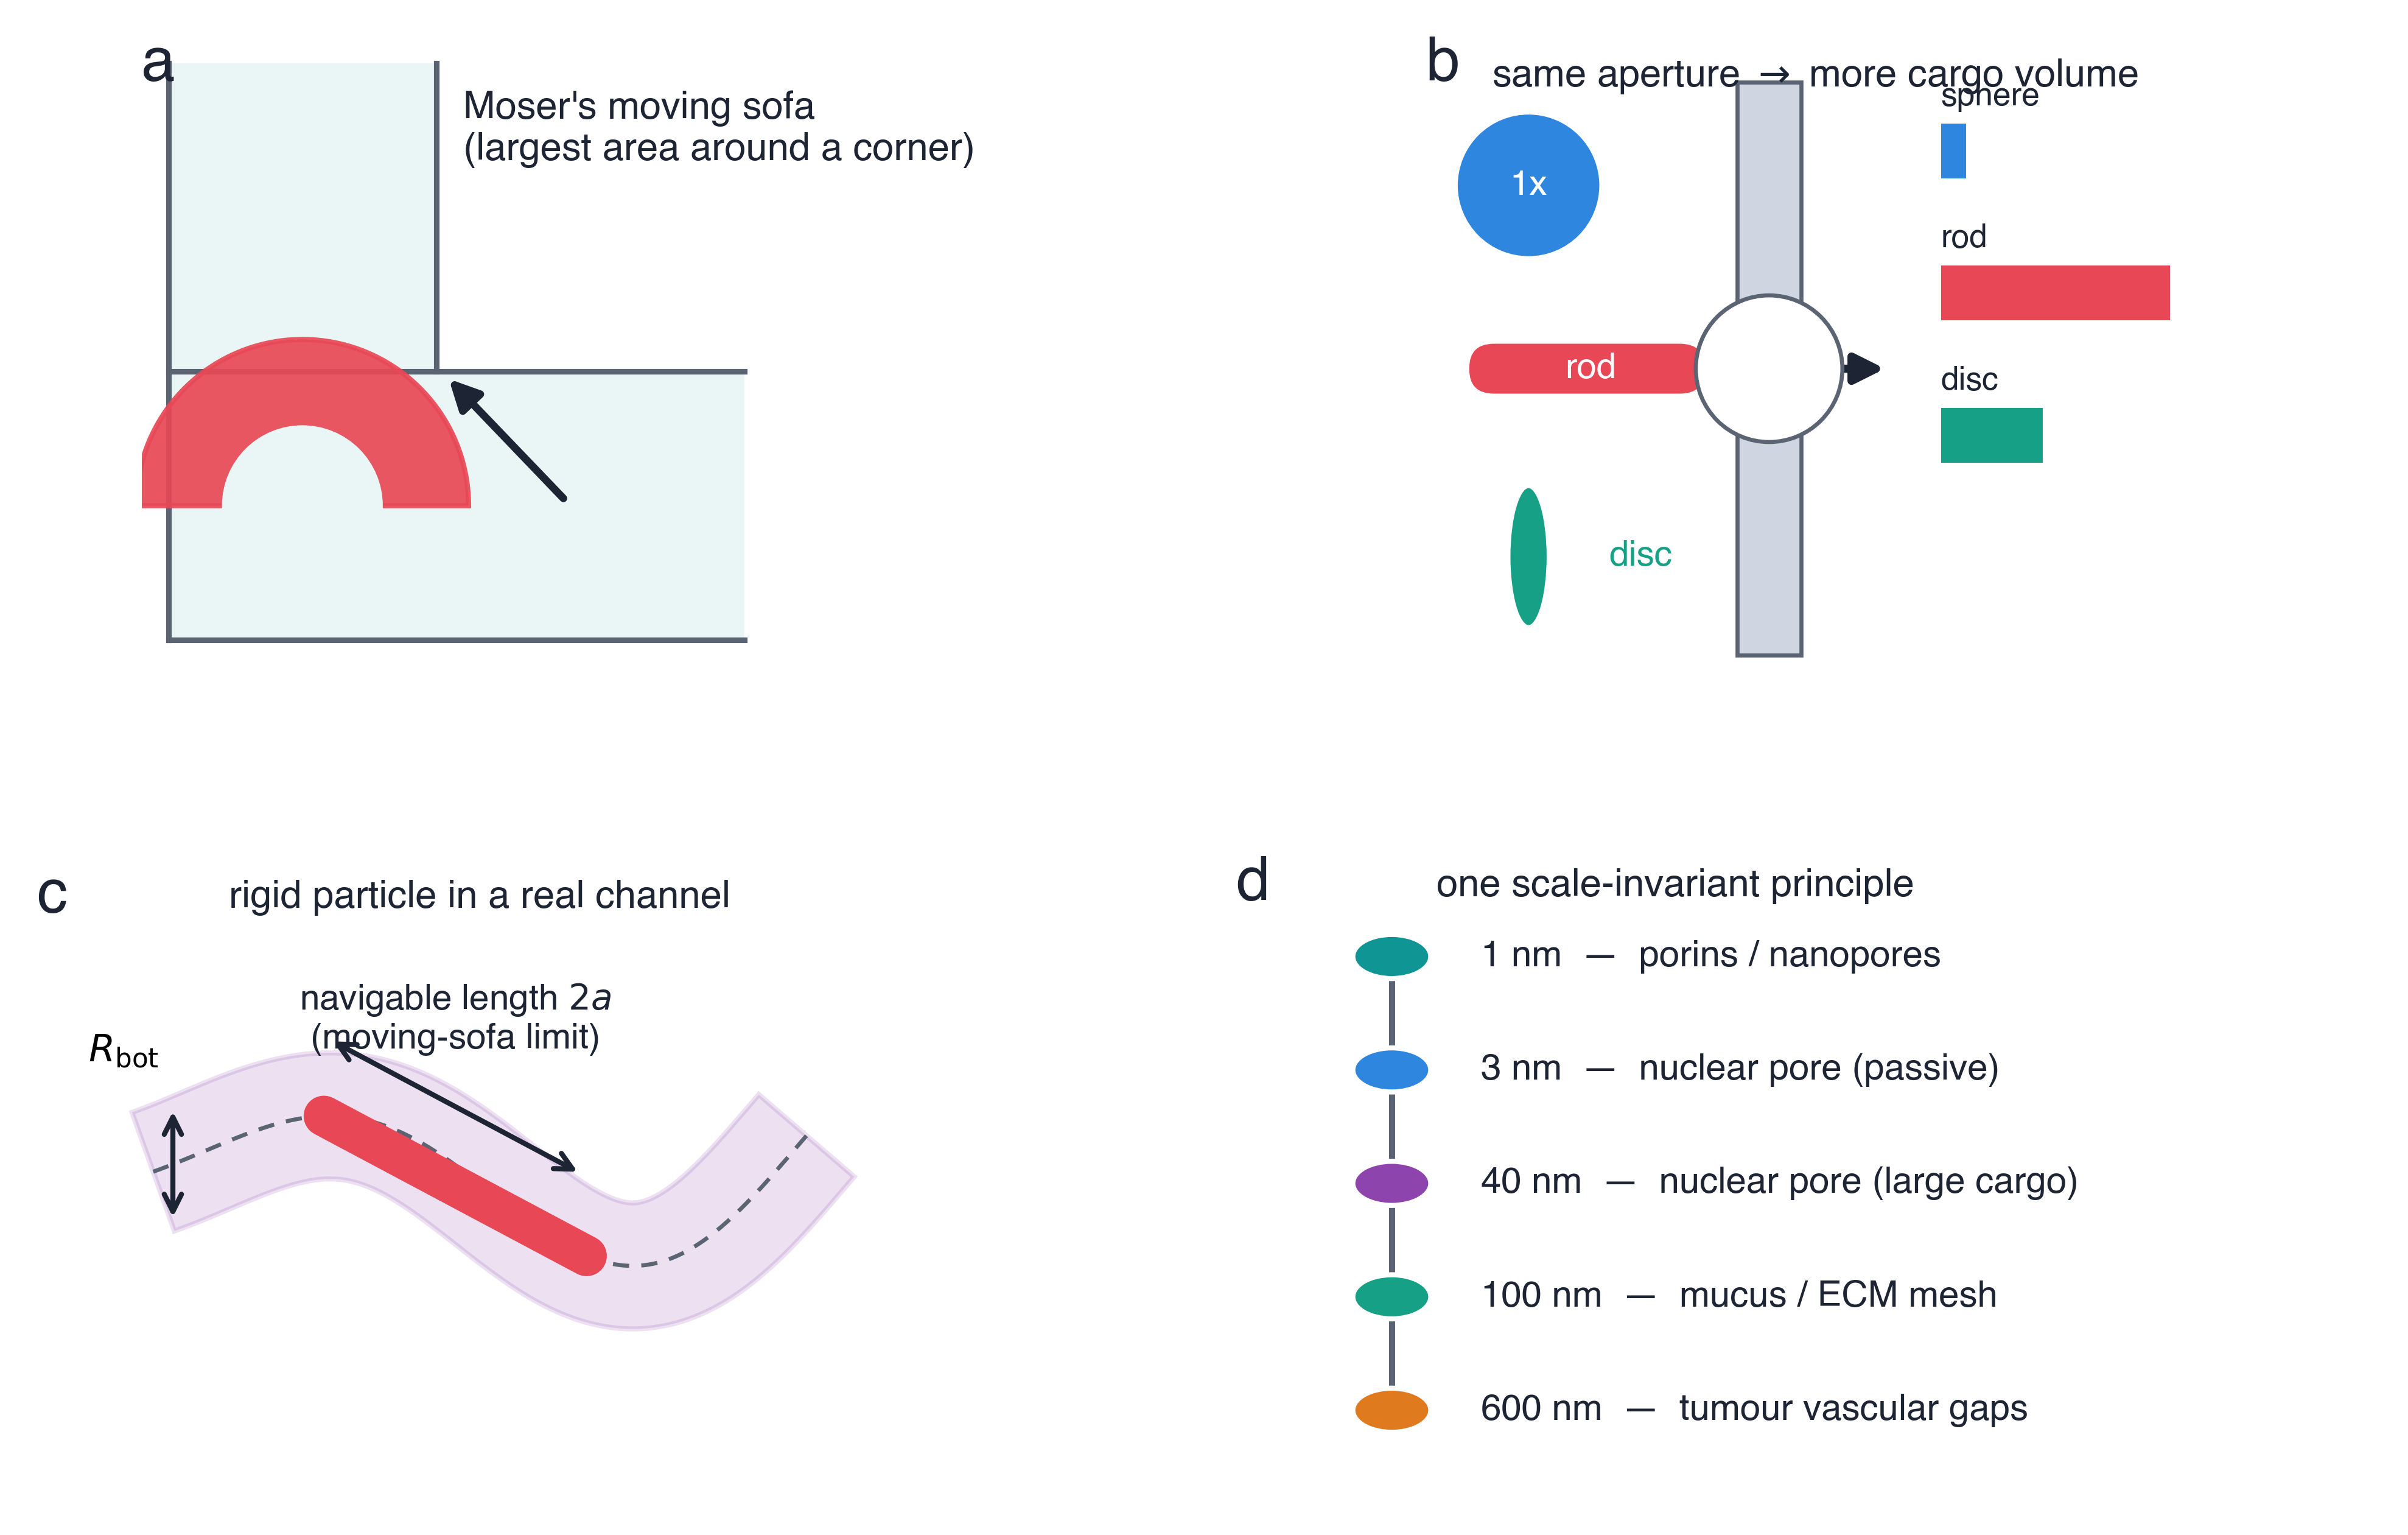
\includegraphics[width=\textwidth]{Figure1_concept.png}
\caption{\textbf{The biological moving-sofa problem.}
(a) Moser's classical problem: the largest rigid area that can round a unit-width
corner is strongly anisotropic and navigation-limited \cite{moser1966,gerver1992,
baek2024}.
(b) For a fixed aperture, an elongated rod or an oblate disc encloses far more
volume than the largest passing sphere.
(c) The two governing constraints on a rigid particle in a real channel: the
transverse cross-section must clear the bottleneck radius $R_{\rm bot}$, while the
navigable length $2a$ is capped by the channel length and its curvature---the
moving-sofa limit.
(d) The principle is scale-invariant, spanning sub-nanometre porins to
micron-scale tissue barriers.}
\label{fig:concept}
\end{figure*}

\begin{figure*}[t]
\centering
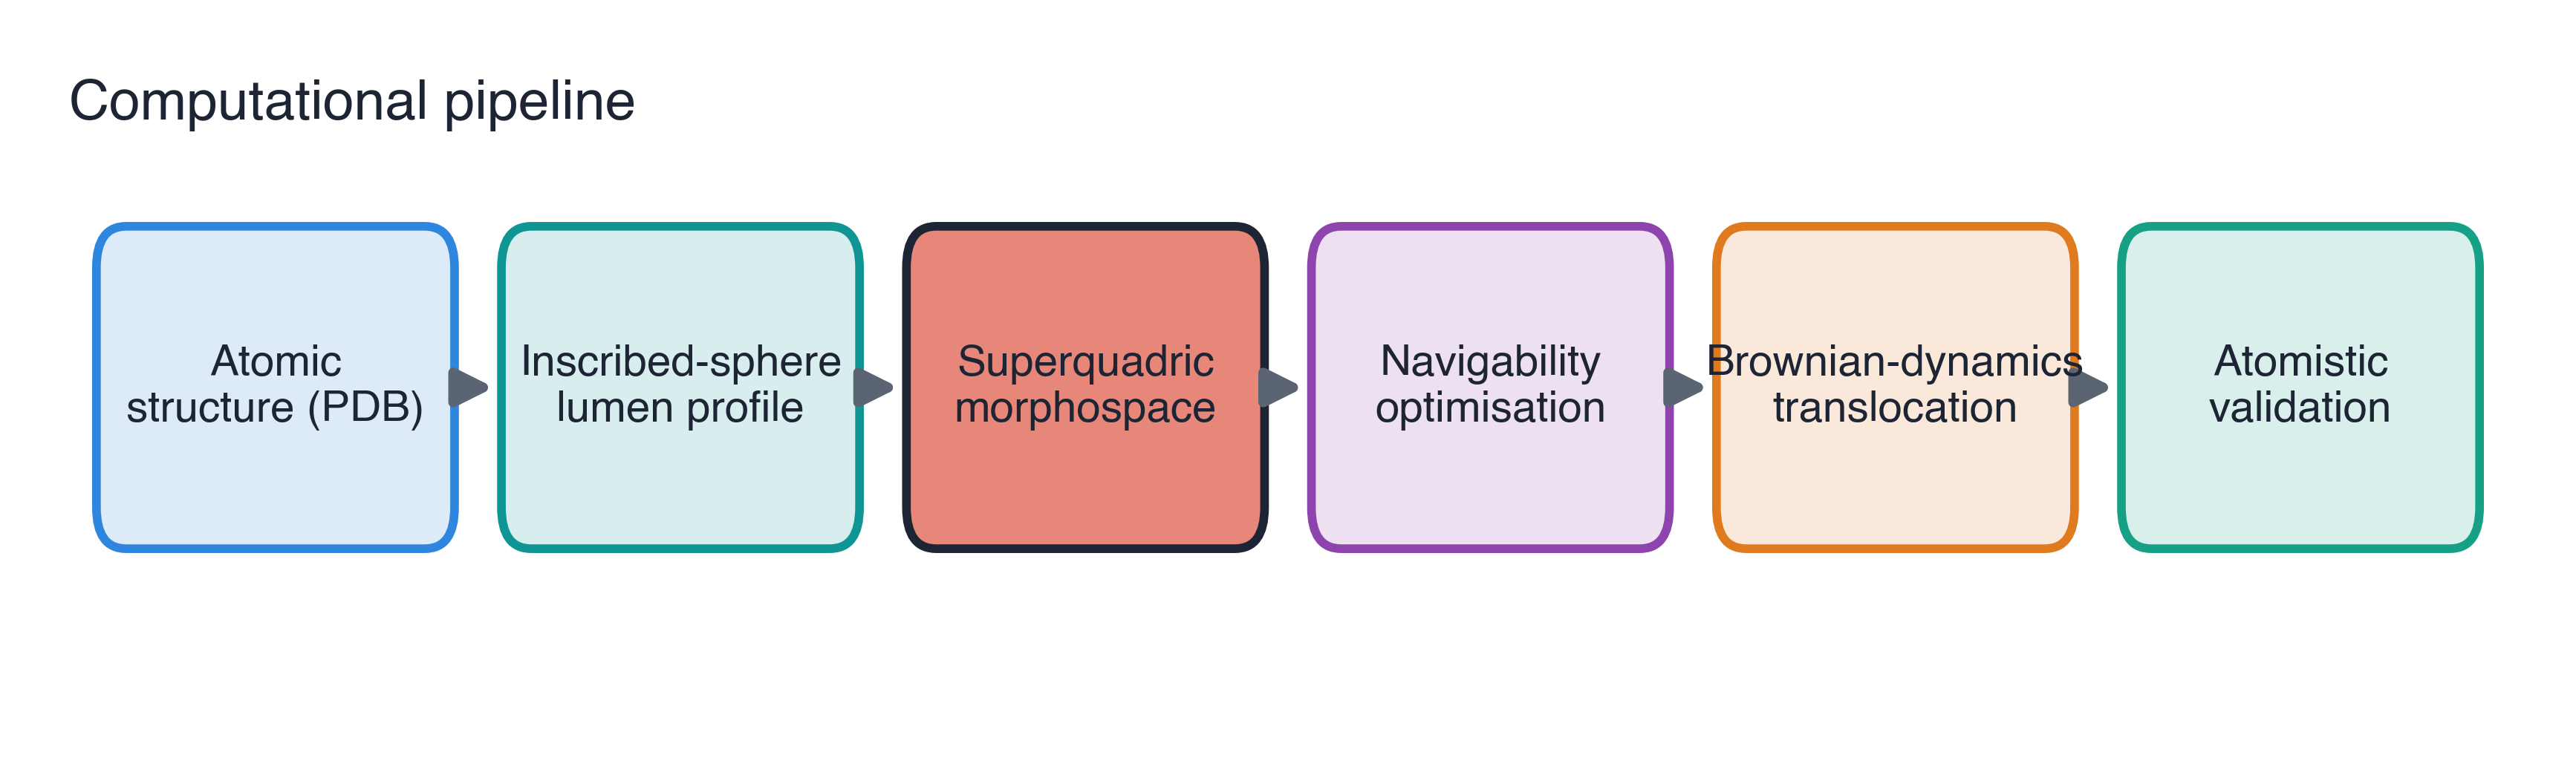
\includegraphics[width=\textwidth]{Figure2_pipeline.png}
\caption{\textbf{Computational pipeline.} Atomistic structures are profiled for
lumen geometry, particles are parameterized in a superquadric morphospace, the
transportable volume is maximized under navigability constraints, and predictions
are stress-tested by Brownian-dynamics translocation and atomistic collision
detection.}
\label{fig:pipeline}
\end{figure*}

%====================================================================
\section{Theoretical framework}

\subsection{Particle family and volume law}

We parameterize rigid particles by the two-exponent superquadric
\cite{barr1981,jaklic2000}, whose surface satisfies
\begin{equation}
\left(\left|\frac{x}{r_x}\right|^{2/\epsilon_2}
+\left|\frac{y}{r_y}\right|^{2/\epsilon_2}\right)^{\epsilon_2/\epsilon_1}
+\left|\frac{z}{c}\right|^{2/\epsilon_1}\le 1 .
\label{eq:superquadric}
\end{equation}
The transport axis is $z$ (half-length $c$); $r_x,r_y$ are transverse
half-widths. The exponent $\epsilon_1$ controls axial squareness
($\epsilon_1=1$ gives ellipsoidal end-caps, $\epsilon_1\!\to\!0$ a flat-ended
cylinder) and $\epsilon_2$ the transverse cross-section ($\epsilon_2=1$ circular,
$\epsilon_2\!\to\!0$ square). This single family continuously interpolates
between spheres, ellipsoids, cylinders/rods, discs and boxes
(Fig.~\ref{fig:morpho}a). Its volume admits the closed form
\begin{equation}
V = 2\,r_x r_y c\,\epsilon_1\epsilon_2\,
B\!\left(\tfrac{\epsilon_1}{2}+1,\epsilon_1\right)
B\!\left(\tfrac{\epsilon_2}{2},\tfrac{\epsilon_2}{2}\right),
\label{eq:volume}
\end{equation}
where $B$ is the Euler beta function \cite{jaklic2000}. We verified
Eq.~\eqref{eq:volume} against direct Monte-Carlo integration over spheres,
prolate and oblate ellipsoids, cylinders and discs, with agreement better than
$0.1\%$ in all cases (Appendix~\ref{app:volume}); the sphere limit reduces
correctly to $\tfrac{4}{3}\pi R^3$. This verification is not incidental: an
incorrect volume law biases the optimum toward boxy shapes and can manufacture a
spurious anisotropy advantage.

\subsection{Transport constraints}

A rigid particle traversing a channel, with its long axis aligned to the local
pore axis, is governed by two geometric constraints.

\emph{(i) Transverse fit.} The maximal cross-section, the $(r_x,r_y,\epsilon_2)$
superellipse, must fit within the aperture. For a circular bottleneck of radius
$R_{\rm bot}$ this requires the circumscribed radius of the cross-section to obey
$\rho_\perp(r_x,r_y,\epsilon_2)\le R_{\rm bot}$; for an elliptical aperture with
half-axes $(p,q)$ the superellipse must be contained in the ellipse, which we
enforce numerically. Aperture anisotropy is quantified by
$\epsilon_{\rm ap}=p/q\ge 1$.

\emph{(ii) Navigable length (the moving-sofa bound).} For a straight channel the
half-length is limited only by the channel length, $a\le L/2$. For a curved
channel the rigid body must round the bend: modelling the lumen as a tube of
radius $R_{\rm bot}$ whose centreline has radius of curvature $\rho$, the longest
straight segment that fits is the chord tangent to the inner wall,
\begin{equation}
a_{\max}=2\sqrt{\rho\,\Delta},\qquad \Delta=R_{\rm bot}-r,
\label{eq:ladder}
\end{equation}
the three-dimensional analogue of the ladder-around-a-corner result and a direct
descendant of the moving-sofa problem (Fig.~\ref{fig:nav}a). Equation
\eqref{eq:ladder} encodes a genuine trade-off: a particle that fills the aperture
($r\!\to\!R_{\rm bot}$, $\Delta\!\to\!0$) has no clearance to turn, so in any
curved channel its navigable length collapses. We relate $\rho$ to the measured
tortuosity $\tau$ (arc length / axial span) through a circular-arc model,
$\tau=(\theta/2)/\sin(\theta/2)$ with $\rho=L_{\rm arc}/\theta$.

\subsection{The optimization}

The transportable cargo volume is maximized,
\begin{equation}
\max_{r_x,r_y,c,\epsilon_1,\epsilon_2}\; V(r_x,r_y,c,\epsilon_1,\epsilon_2)
\quad\text{s.t. (i) and (ii)},
\label{eq:opt}
\end{equation}
and benchmarked against the largest passing sphere, of radius
$R_s=\min(R_{\rm bot},L/2)$ and volume $\tfrac{4}{3}\pi R_s^3$ (a sphere cannot
traverse a barrier shorter than its diameter). The capacity gain is
$G=V_{\rm opt}/V_{\rm sphere}$. Because both volumes scale identically with
absolute size, $G$ is dimensionless and depends only on the shape ratios
$L/R_{\rm bot}$, $\tau$ and $\epsilon_{\rm ap}$---the origin of the
scale-invariance exploited in Sec.~\ref{sec:meso}.

%====================================================================
\section{Atomistic channel geometry}

We selected four canonical, structurally well-resolved biological nanopores that
span the relevant geometric range while forming a homogeneous family of genuine
transport channels: the staphylococcal $\alpha$-hemolysin heptamer
(PDB 7AHL) \cite{song1996ahl}, the mitochondrial porin VDAC1 (3EMN)
\cite{ujwal2008vdac}, the connexin-26 gap-junction connexon (2ZW3)
\cite{maeda2009connexin}, and the mycobacterial porin MspA (1UUN, biological
octamer) \cite{faller2004mspa}. Heavy-atom coordinates were assigned Bondi van
der Waals radii \cite{bondi1964}.

The pore axis, centreline and radius profile $R(z)$ were obtained by a
re-implementation of the \textsc{hole} inscribed-sphere algorithm
\cite{smart1996hole}: the channel axis is found by a cylinder fit refined to
maximize the enclosed lumen length, and the largest probe sphere is propagated
continuously along the axis with an enclosure criterion that prevents escape into
bulk solvent (Sec.~\ref{sec:methods}). The recovered constrictions
(Fig.~\ref{fig:geom}; Table~\ref{tab:channels}) reproduce known values: all four
pores have minimum diameters near $\SI{1.0}{nm}$, and the recovered lengths
($4.8$--$\SI{10.0}{nm}$), funnel/goblet asymmetries (MspA), and the pronounced
tortuosity of VDAC1 ($\tau=1.56$, reflecting the N-terminal helix that lines and
bends its lumen) are all consistent with the structures. The remaining three
channels are essentially straight ($\tau\le 1.07$), establishing that real
$\beta$-barrel and pore-forming-toxin channels offer little intrinsic curvature
---the elongation budget is set primarily by channel length.

\begin{figure*}[t]
\centering
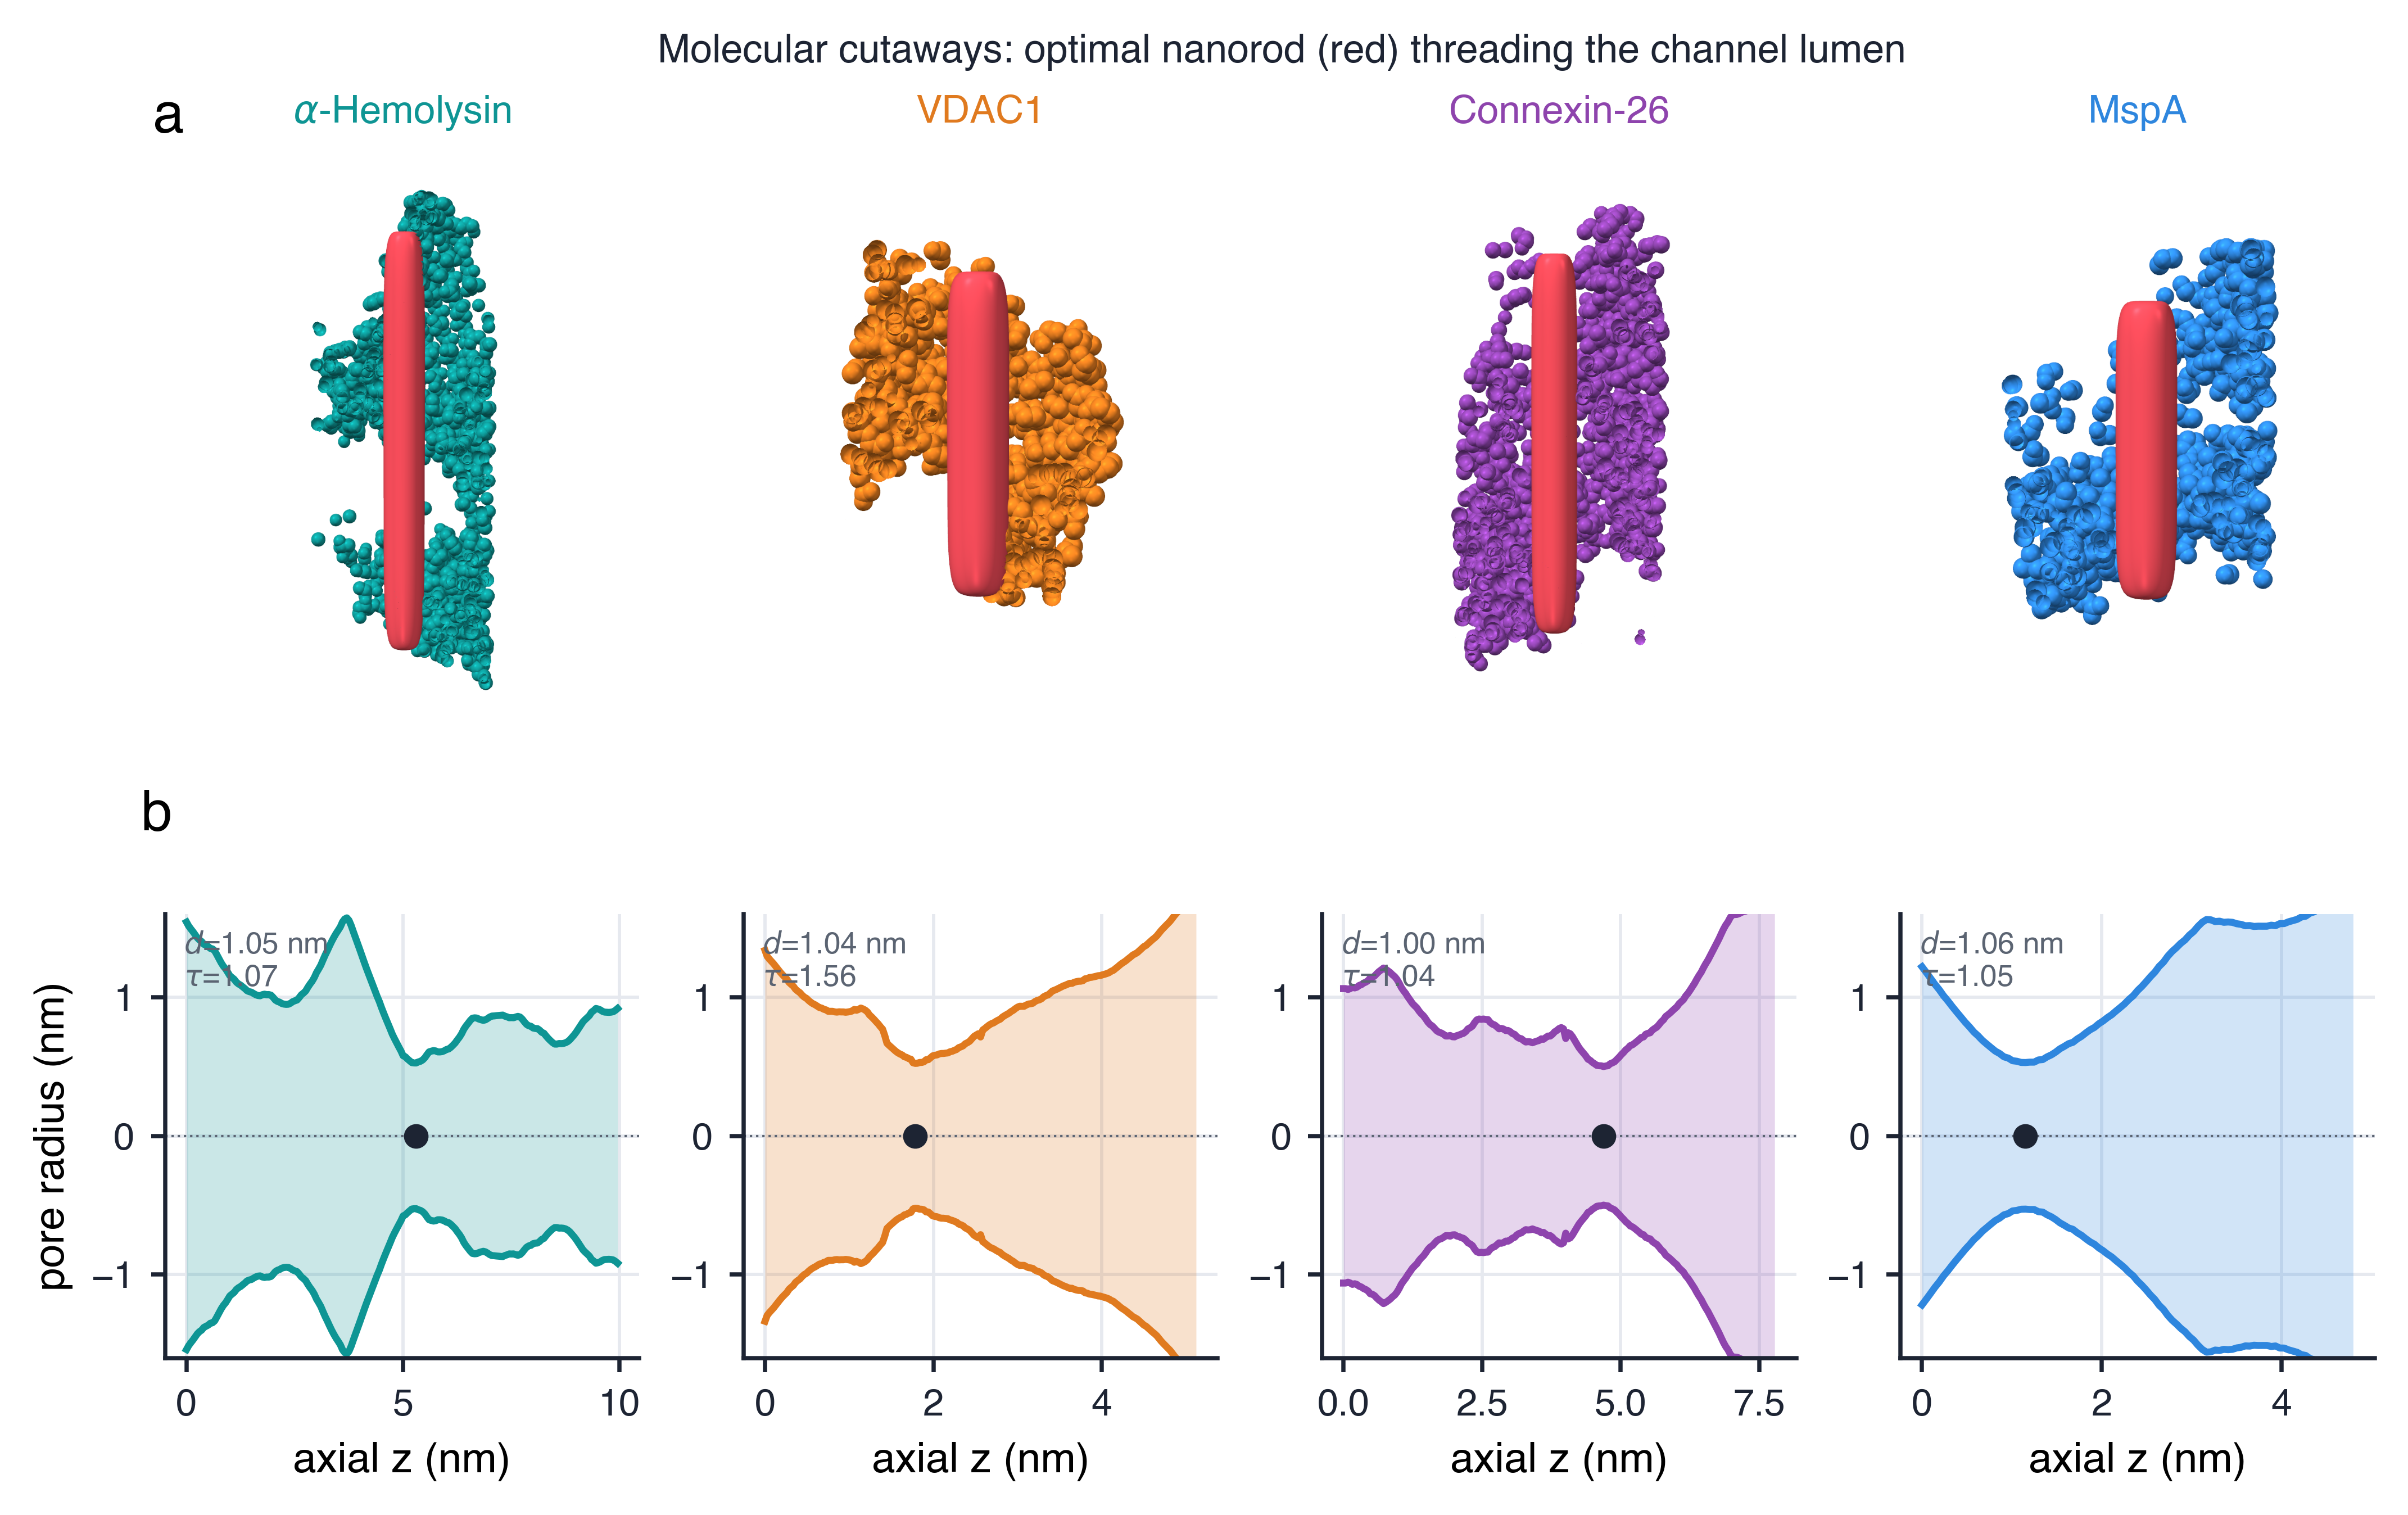
\includegraphics[width=\textwidth]{Figure3_geometry.png}
\caption{\textbf{Atomistic lumen geometry and the optimal nanorod.}
(a) Molecular cutaways (space-filling protein, coloured and clipped to expose
the lumen) with the optimized nanorod (red) threading each channel.
(b) Inscribed-sphere pore-radius profiles $R(z)$; the bottleneck (dot), minimum
diameter $d$ and tortuosity $\tau$ are annotated. All four constrictions are
near $\SI{1}{nm}$.}
\label{fig:geom}
\end{figure*}

\begin{table*}[t]
\caption{Structural and geometric parameters of the four channels, extracted
\emph{de novo} from atomic coordinates, and the resulting validated capacity
gain. $d$, minimum pore diameter; $L$, lumen length; $\tau$, centreline
tortuosity; $\epsilon_{\rm ap}$, aperture anisotropy; $V_{\rm sph}$, volume of
the largest passing sphere; $a/R_{\rm bot}$, validated optimal aspect ratio;
$G$, transportable-volume gain.}
\label{tab:channels}
\begin{ruledtabular}
\begin{tabular}{lccccccccc}
Channel & PDB & atoms & $d$ (nm) & $L$ (nm) & $\tau$ & $\epsilon_{\rm ap}$
 & $V_{\rm sph}$ (nm$^3$) & $a/R_{\rm bot}$ & $G$ \\
\colrule
$\alpha$-Hemolysin & 7AHL & 16389 & 1.05 & 10.0 & 1.07 & 2.40 & 0.61 & 13.3 & $\mathbf{19.4}$ \\
VDAC1              & 3EMN & 2189  & 1.04 & 5.1  & 1.56 & 1.77 & 0.60 & 6.9  & $\mathbf{10.0}$ \\
Connexin-26        & 2ZW3 & 9834  & 1.00 & 7.8  & 1.04 & 1.78 & 0.52 & 10.9 & $\mathbf{15.9}$ \\
MspA               & 1UUN & 11032 & 1.06 & 4.8  & 1.05 & 1.78 & 0.62 & 6.4  & $\mathbf{9.3}$ \\
\end{tabular}
\end{ruledtabular}
\end{table*}

%====================================================================
\section{Optimal transport shapes and capacity gains}

Solving Eq.~\eqref{eq:opt} for each channel returns the same kind of optimum: a
\emph{round-cross-section nanorod}. In every case the optimizer drives
$\epsilon_2\to 1$ (a circular cross-section, which alone maximizes area inside a
circular aperture) and $\epsilon_1\to 0.2$ (a flat-ended cylinder, which
maximizes axial filling), and it places the transverse radius right at the
constriction (Fig.~\ref{fig:morpho}b). Boxy, high-exponent shapes, which a naive
or mis-normalized volume law would favour, are rejected outright. This is one
reason the verified volume law of Eq.~\eqref{eq:volume} matters: with the wrong
prefactor the optimization would invent an anisotropy advantage that is not
there.

The capacity gains are large and, importantly, \emph{not} universal constants but
quantities that track each channel's geometry. The atomistically validated gains
(Sec.~\ref{sec:valid}, Fig.~\ref{fig:gains}) are $19.4\times$
($\alpha$-hemolysin), $15.9\times$ (connexin-26), $10.0\times$ (VDAC1) and
$9.3\times$ (MspA). To leading order a cylinder of radius $R_{\rm bot}$ and length
$2a$ improves on the sphere by $G\simeq\tfrac32\,(a/R_{\rm bot})$, so the gain is
governed by the achievable aspect ratio, which in turn is set by the channel
length-to-radius ratio $L/2R_{\rm bot}$ (Fig.~\ref{fig:gains}c). The longest,
narrowest channel ($\alpha$-hemolysin, $L/2R_{\rm bot}\approx 9.5$) yields the
largest gain; the shortest (MspA) the smallest. This monotonic, mechanistic
dependence---rather than a single headline number---is the central quantitative
result.

\begin{figure*}[t]
\centering
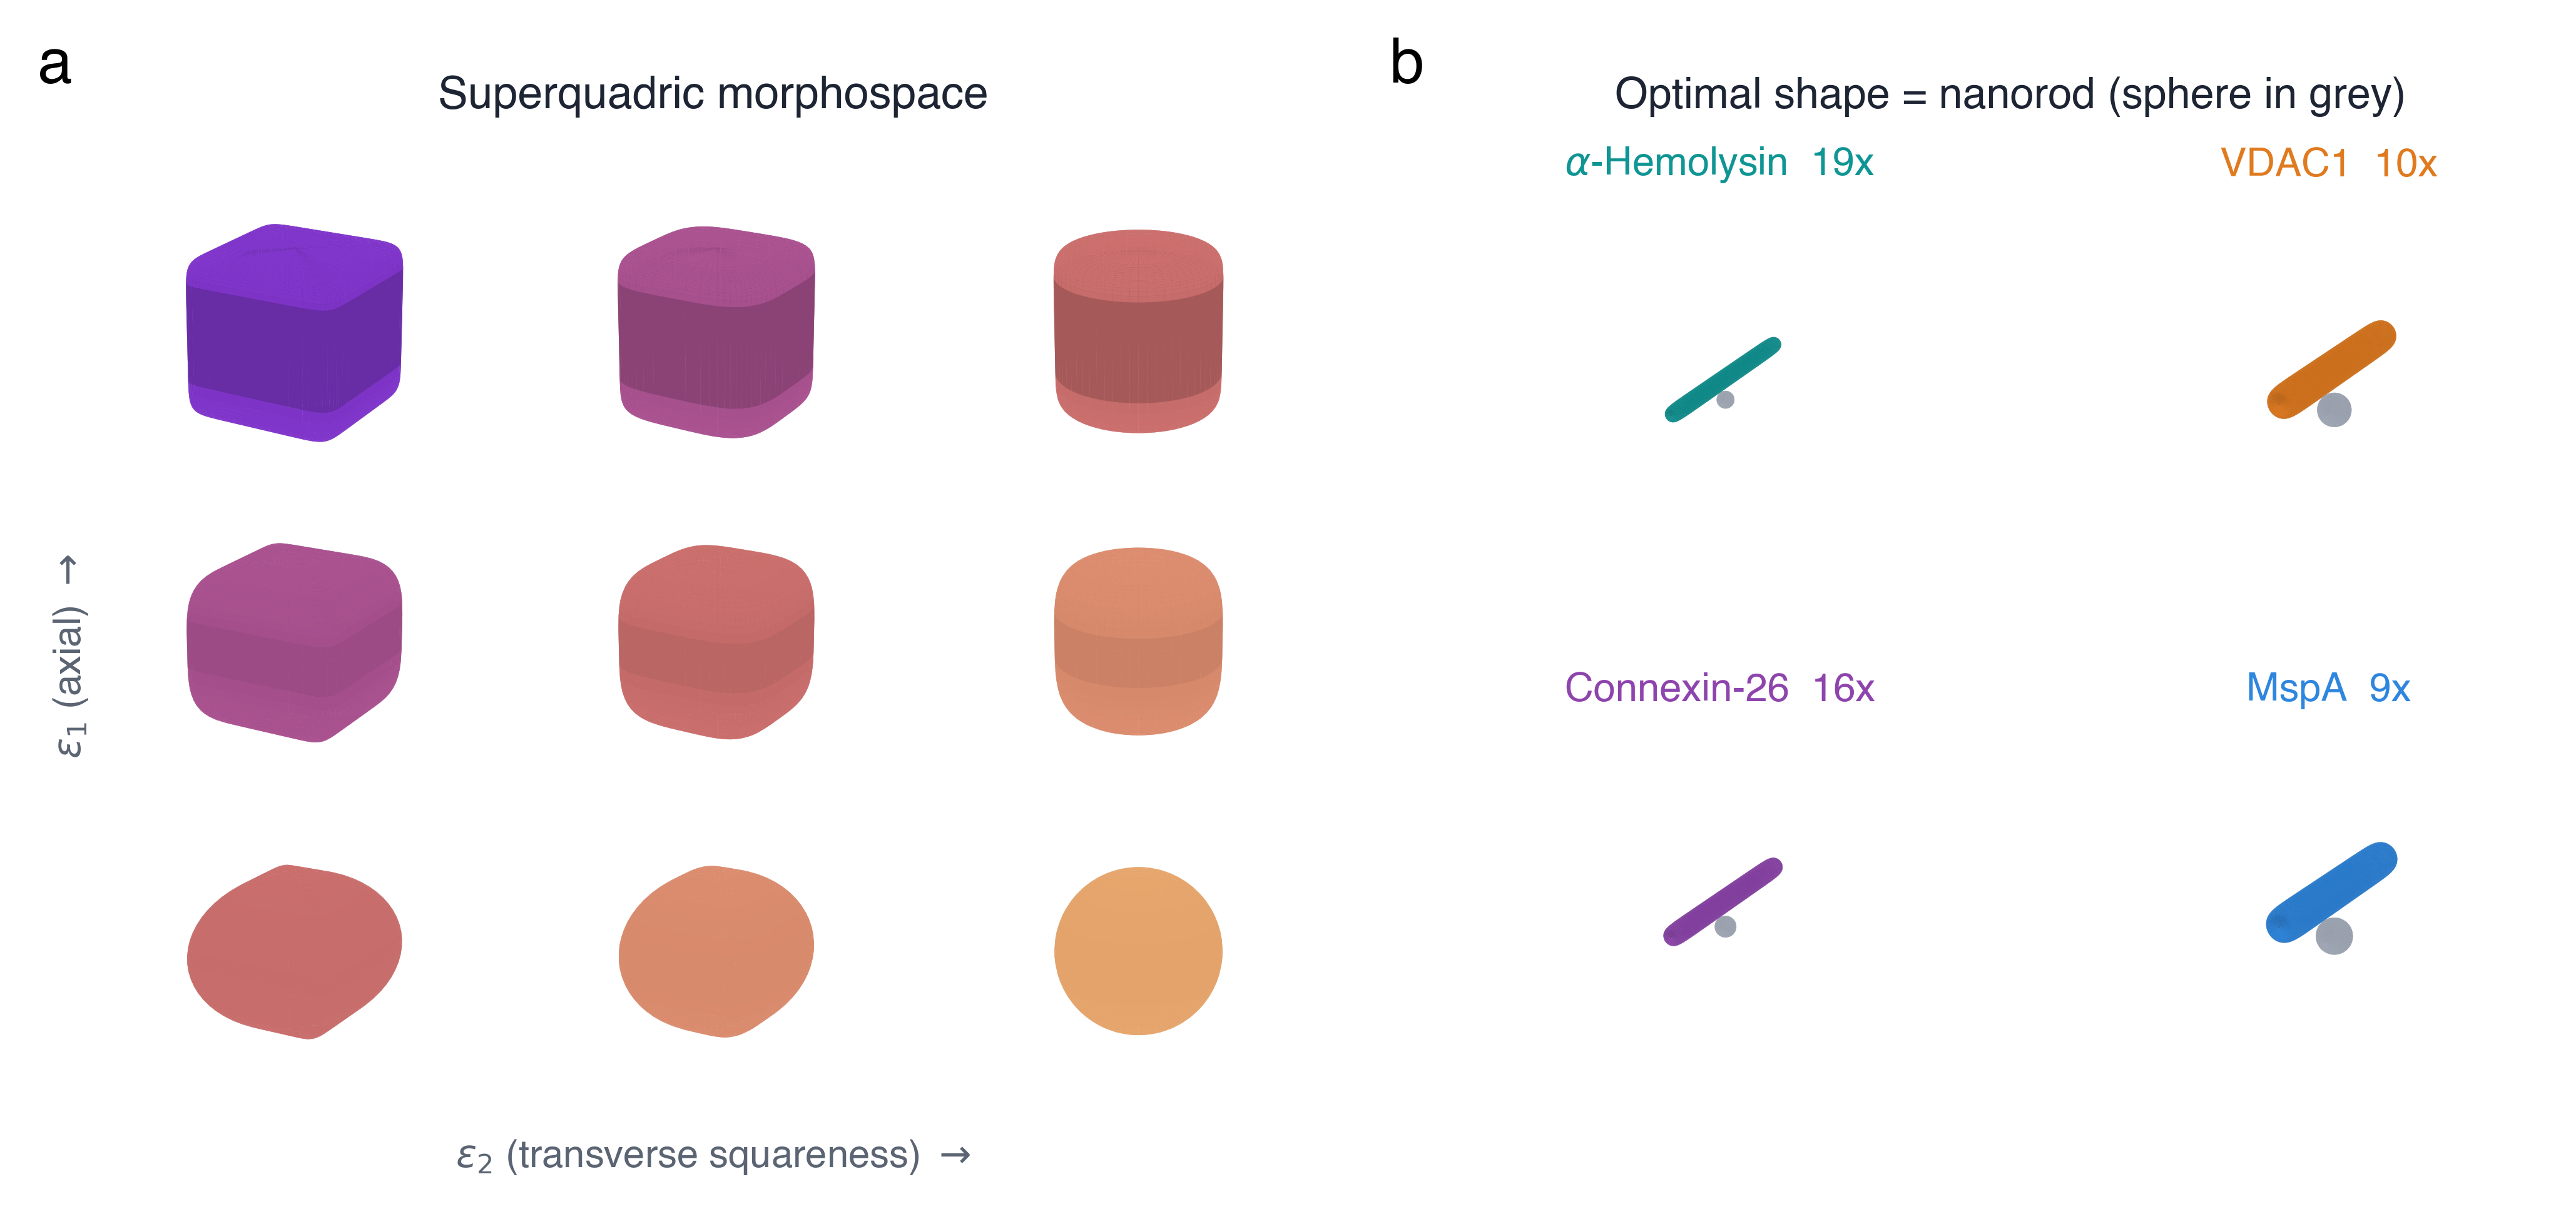
\includegraphics[width=\textwidth]{Figure4_morphospace.png}
\caption{\textbf{Superquadric morphospace and channel optima.}
(a) The two-exponent superquadric family spans spheres, cylinders, discs and
boxes as $(\epsilon_1,\epsilon_2)$ vary.
(b) For all four channels the optimum is a round-cross-section nanorod
(coloured) carrying $9$--$19\times$ the volume of the largest passing sphere
(grey).}
\label{fig:morpho}
\end{figure*}

\begin{figure*}[t]
\centering
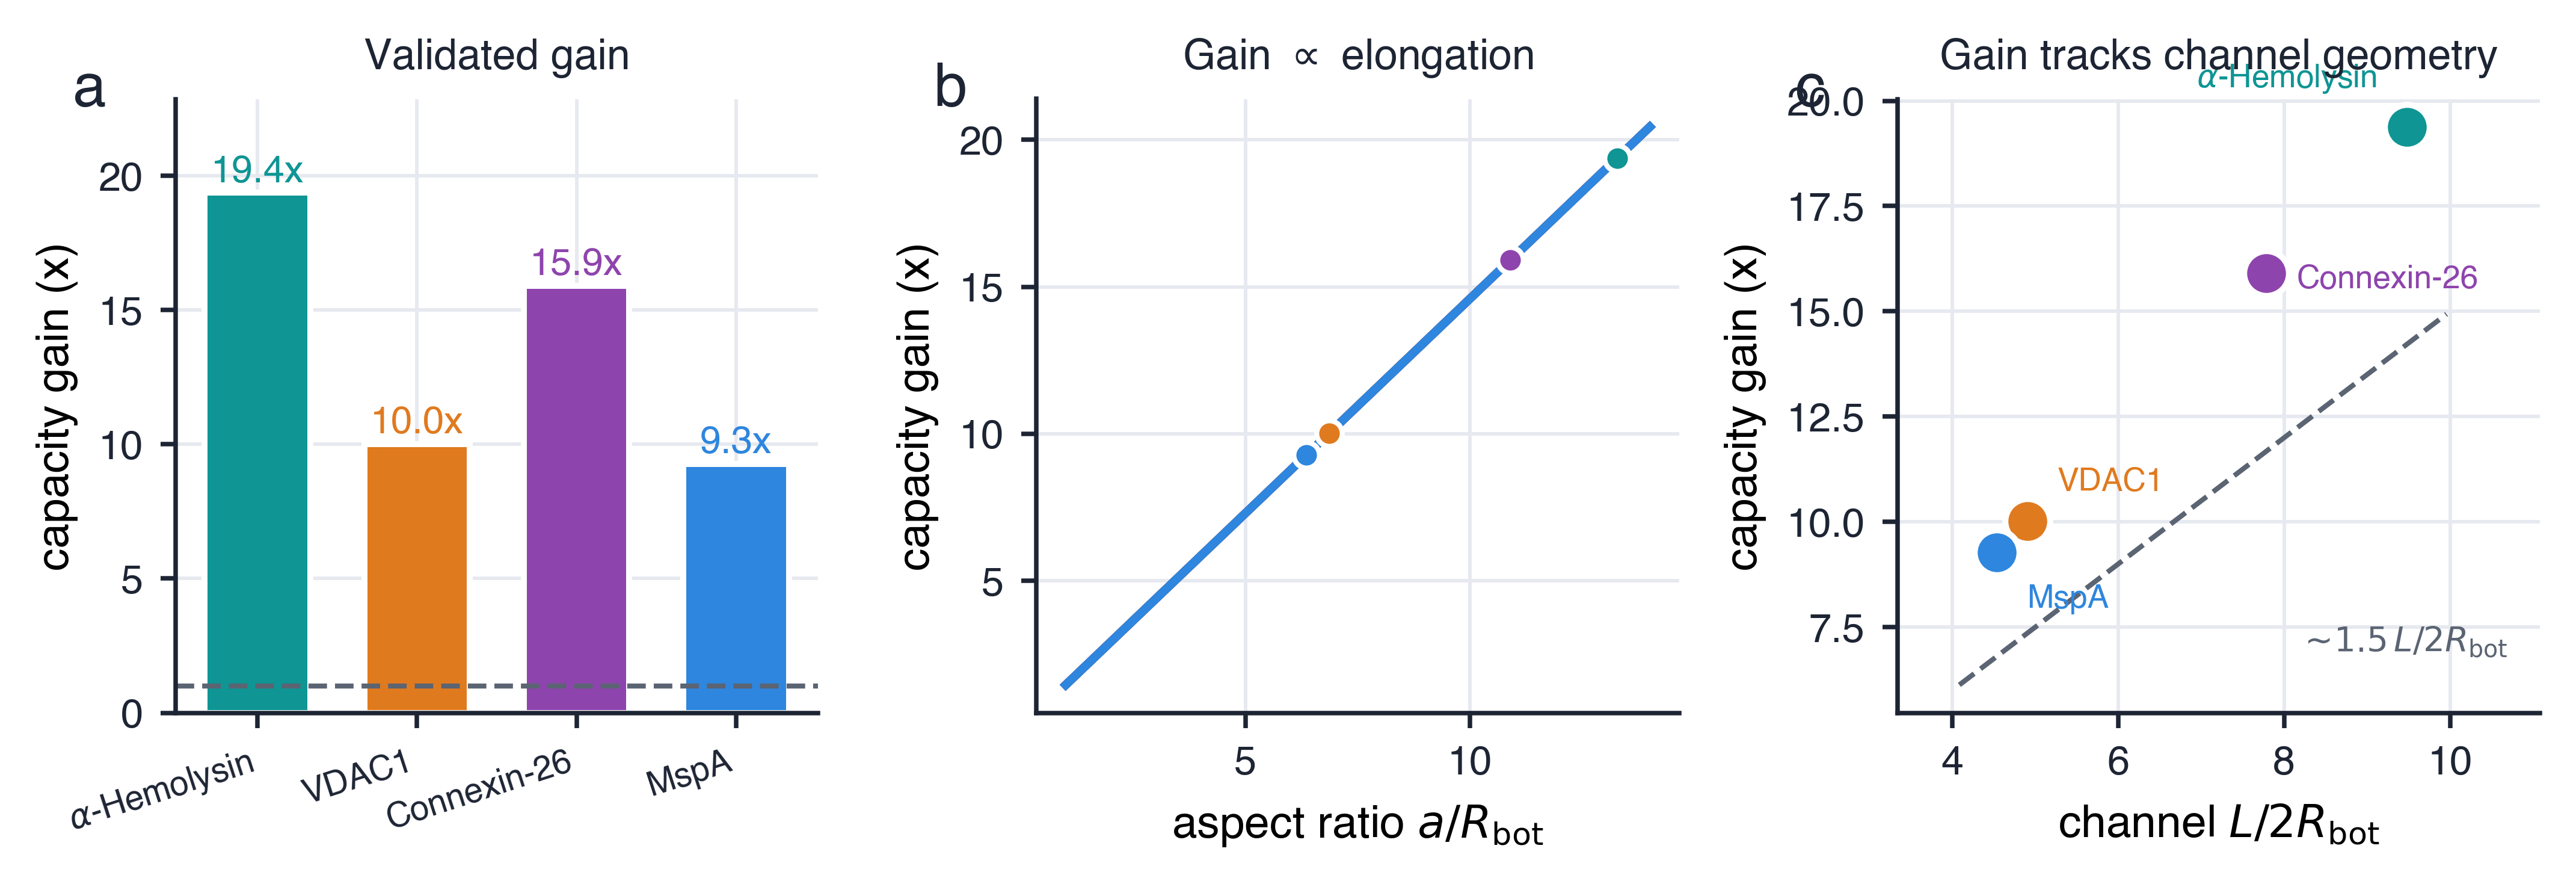
\includegraphics[width=\textwidth]{Figure5_gains.png}
\caption{\textbf{Capacity gains.}
(a) Atomistically validated transportable-volume gain per channel.
(b) Gain versus allowed aspect ratio $a/R_{\rm bot}$; markers denote the
collision-validated optimum.
(c) The gain tracks the channel length-to-radius ratio, following the cylinder
estimate $G\simeq\tfrac32\,L/2R_{\rm bot}$ (dashed).}
\label{fig:gains}
\end{figure*}

%====================================================================
\section{Atomistic validation}
\label{sec:valid}

Every prediction above rests on an analytic optimization, so we tested it
independently by brute-force collision detection against the atomic coordinates,
using no part of the volume law or the aperture constraint
(Fig.~\ref{fig:valid}). Two orthogonal checks were performed. First, a probe of
increasing radius placed on the pore axis at the constriction loses clearance
exactly at $R_{\rm bot}$ (Fig.~\ref{fig:valid}a), confirming that the extracted
bottleneck is the binding transverse constraint. Second, a rigid cylinder of
fixed sub-constriction radius and growing half-length, swept along the lumen over
a search of position and orientation, remains collision-free up to a
channel-specific navigable length $a_{\rm nav}$ (Fig.~\ref{fig:valid}b). The
resulting validated aspect ratios and gains (Table~\ref{tab:channels}) define the
markers used throughout and confirm the analytic optima; the throttling of
$a_{\rm nav}$ in the tortuous VDAC1 lumen, relative to straight channels of
similar length, is recovered directly from the atoms. A cross-sectional view
(Fig.~\ref{fig:valid}c) confirms the optimal nanorod sits collision-free within
the lumen.

\begin{figure*}[t]
\centering
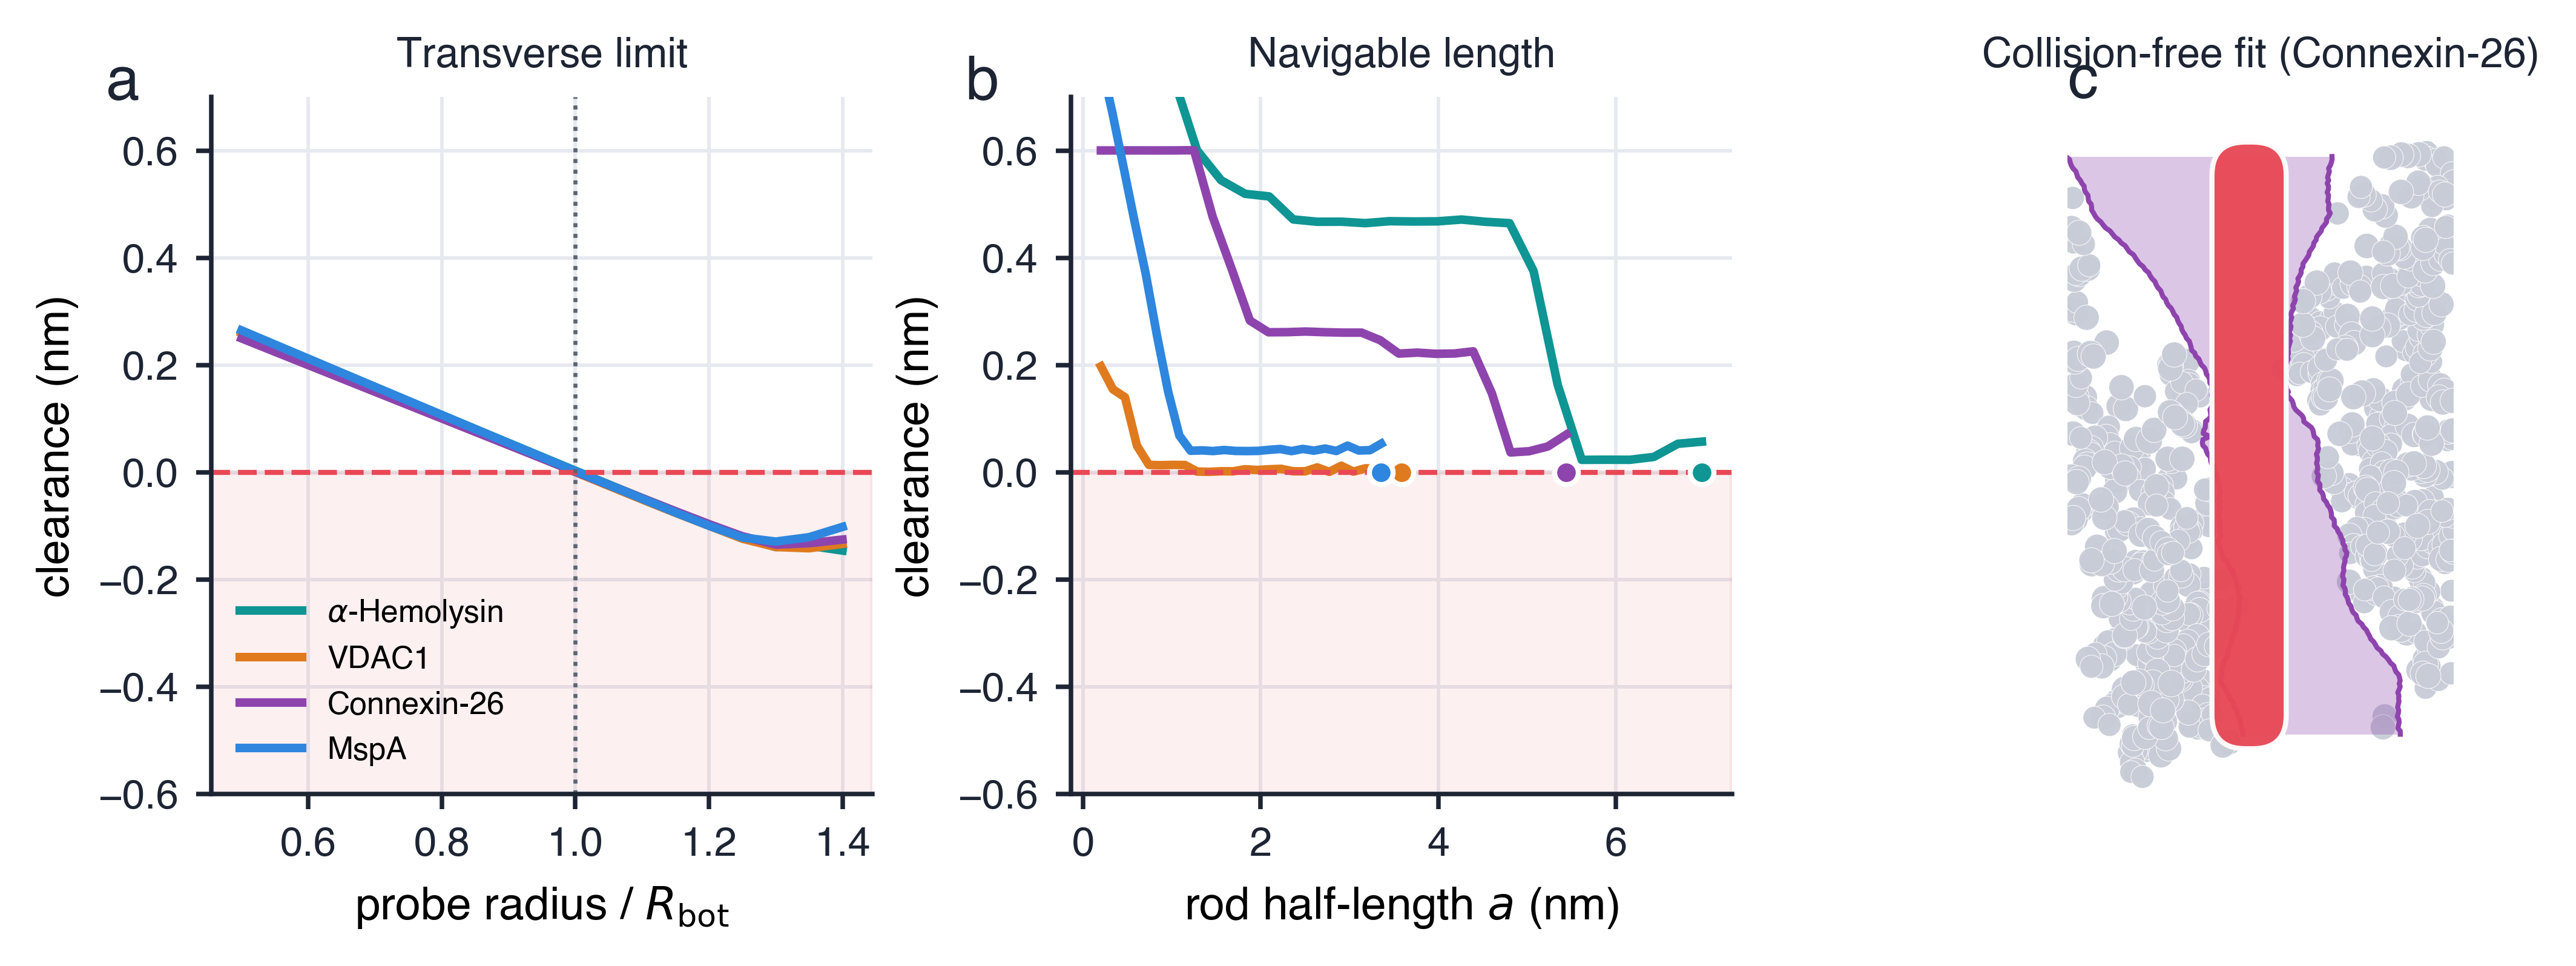
\includegraphics[width=\textwidth]{Figure9_validation.png}
\caption{\textbf{Atomistic collision validation.}
(a) Probe clearance versus radius: all channels lose clearance at the extracted
$R_{\rm bot}$ (transverse limit).
(b) Clearance versus rod half-length; the zero-crossing (markers) is the
atomistically measured navigable length $a_{\rm nav}$.
(c) Cross-section confirming the optimal nanorod (red) fits the connexin-26 lumen
without clashes.}
\label{fig:valid}
\end{figure*}

%====================================================================
\section{Navigability and the design map}
\label{sec:nav}

The elongation that powers these gains is ultimately limited by navigability.
Equation~\eqref{eq:ladder} shows that curvature throttles the achievable aspect
ratio (Fig.~\ref{fig:nav}b): the idealized smooth-bend bound falls steeply with
tortuosity, while the atomistically measured navigable lengths
(Sec.~\ref{sec:valid}) lie above it because the small residual tortuosity of real
``straight'' channels ($\tau\!\approx\!1.05$) is wall roughness rather than a
coherent bend. The genuinely tortuous channel, VDAC1, is the outlier whose
achievable aspect ratio---and hence gain---is visibly suppressed relative to
straight channels of comparable length.

These dependencies collapse onto a compact \emph{design map}
(Fig.~\ref{fig:nav}c): the capacity gain as a function of the two levers a
designer can target, the achievable aspect ratio $a/R_{\rm bot}$ (set by length
and tortuosity) and the aperture anisotropy $\epsilon_{\rm ap}$ (which lets a
flattened particle exploit the wide direction of a slit). Gain rises smoothly
from unity (isotropic, short channels) toward $\sim\!25\times$ (long and/or
slit-like channels). The four nanopores populate the moderate-anisotropy,
high-aspect-ratio region; the map immediately predicts where engineered or
mesoscale channels would lie.

\begin{figure*}[t]
\centering
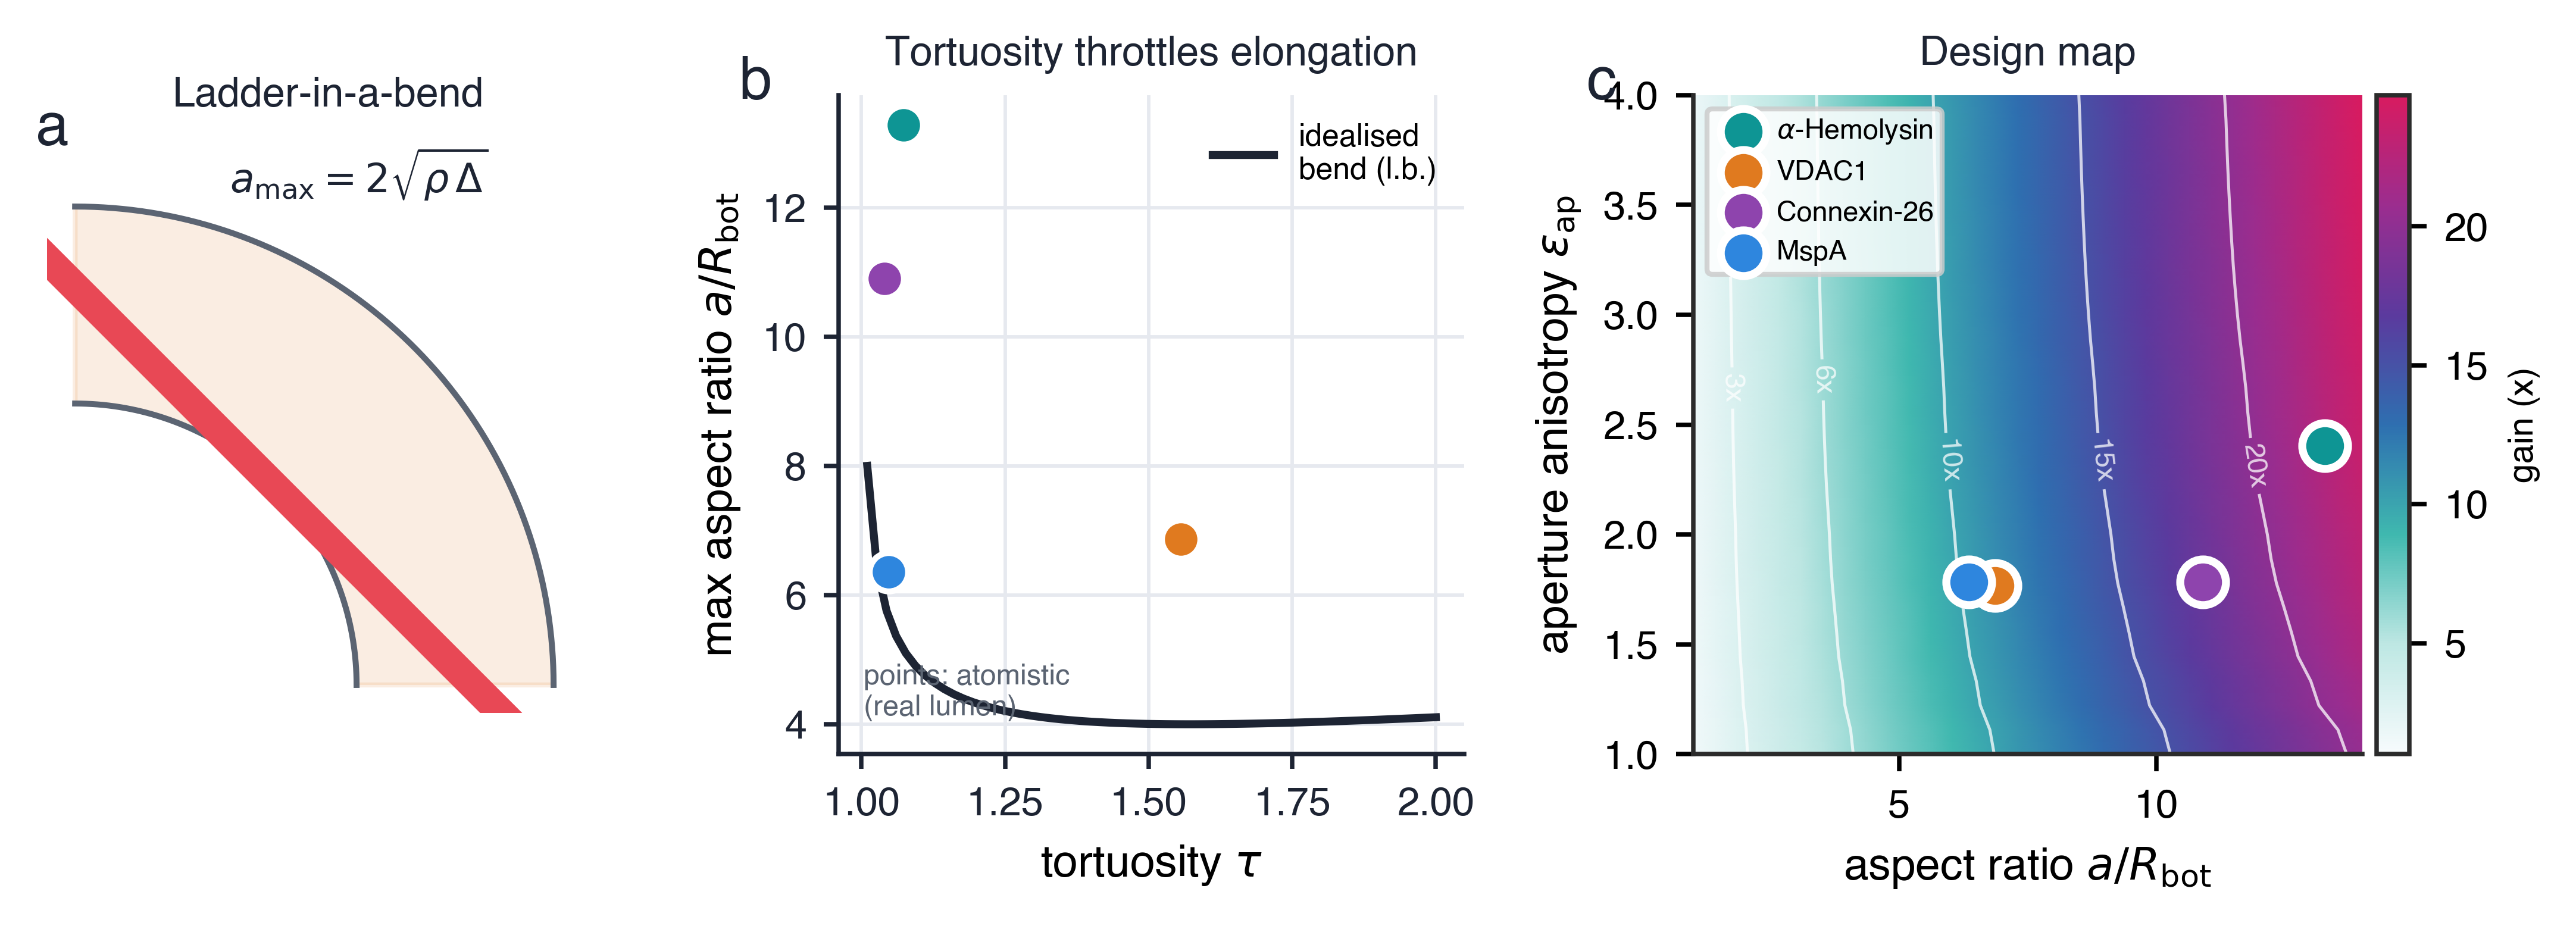
\includegraphics[width=\textwidth]{Figure6_navigability.png}
\caption{\textbf{Navigability physics and the design map.}
(a) The moving-sofa/ladder bound: the longest rigid segment in a bent tube,
$a_{\max}=2\sqrt{\rho\Delta}$.
(b) Tortuosity throttles the achievable aspect ratio; the curve is the idealized
smooth-bend bound (a lower bound), points are atomistic measurements on the real
lumens.
(c) Design map: transportable-volume gain versus aspect ratio and aperture
anisotropy, with the four channels overlaid.}
\label{fig:nav}
\end{figure*}

%====================================================================
\section{Brownian-dynamics translocation}

Geometric capacity is necessary but not sufficient: a high-capacity shape is
useful only if it can actually translocate. We therefore computed, for each
channel, the entropic potential of mean force (PMF) $G(z)$ along the pore axis
for a sphere, the optimal rod and an oblate disc, by Monte-Carlo sampling of
collision-free rigid configurations (transverse offset and orientation) against
the atomic coordinates---a Fick--Jacobs construction \cite{zwanzig1992}. We then
integrated the overdamped Langevin equation on $G(z)$ with absorbing mouths and
an external drive $f$, yielding translocation probabilities and mean
first-passage times (Fig.~\ref{fig:bd}).

The simulations make three points. First, oblate \emph{discs are sterically
excluded} from all four circular pores: their PMF barrier saturates the sampling
limit and their translocation probability is essentially zero
(Fig.~\ref{fig:bd}a,b). Discs therefore help only at slit-like or short, wide
apertures, not at circular pores, a conclusion that returns at the mesoscale
(Sec.~\ref{sec:meso}). Second, the optimal nanorod still translocates: it crosses
with finite probability under modest drive (Fig.~\ref{fig:bd}c), and its entropic
barrier is comparable to, or lower than, that of the maximal sphere
(Fig.~\ref{fig:bd}b,d). The reason is intuitive once stated: the rod sits below
the constriction in its transverse dimension, so it threads at least as easily as
a sphere, while its length is what supplies the extra volume. Third, putting these
together, the move from sphere to rod buys an order of magnitude in cargo while
leaving the translocation barrier essentially unchanged (Fig.~\ref{fig:bd}d). The
capacity advantage, in other words, does not come at the expense of getting
through.

\begin{figure*}[t]
\centering
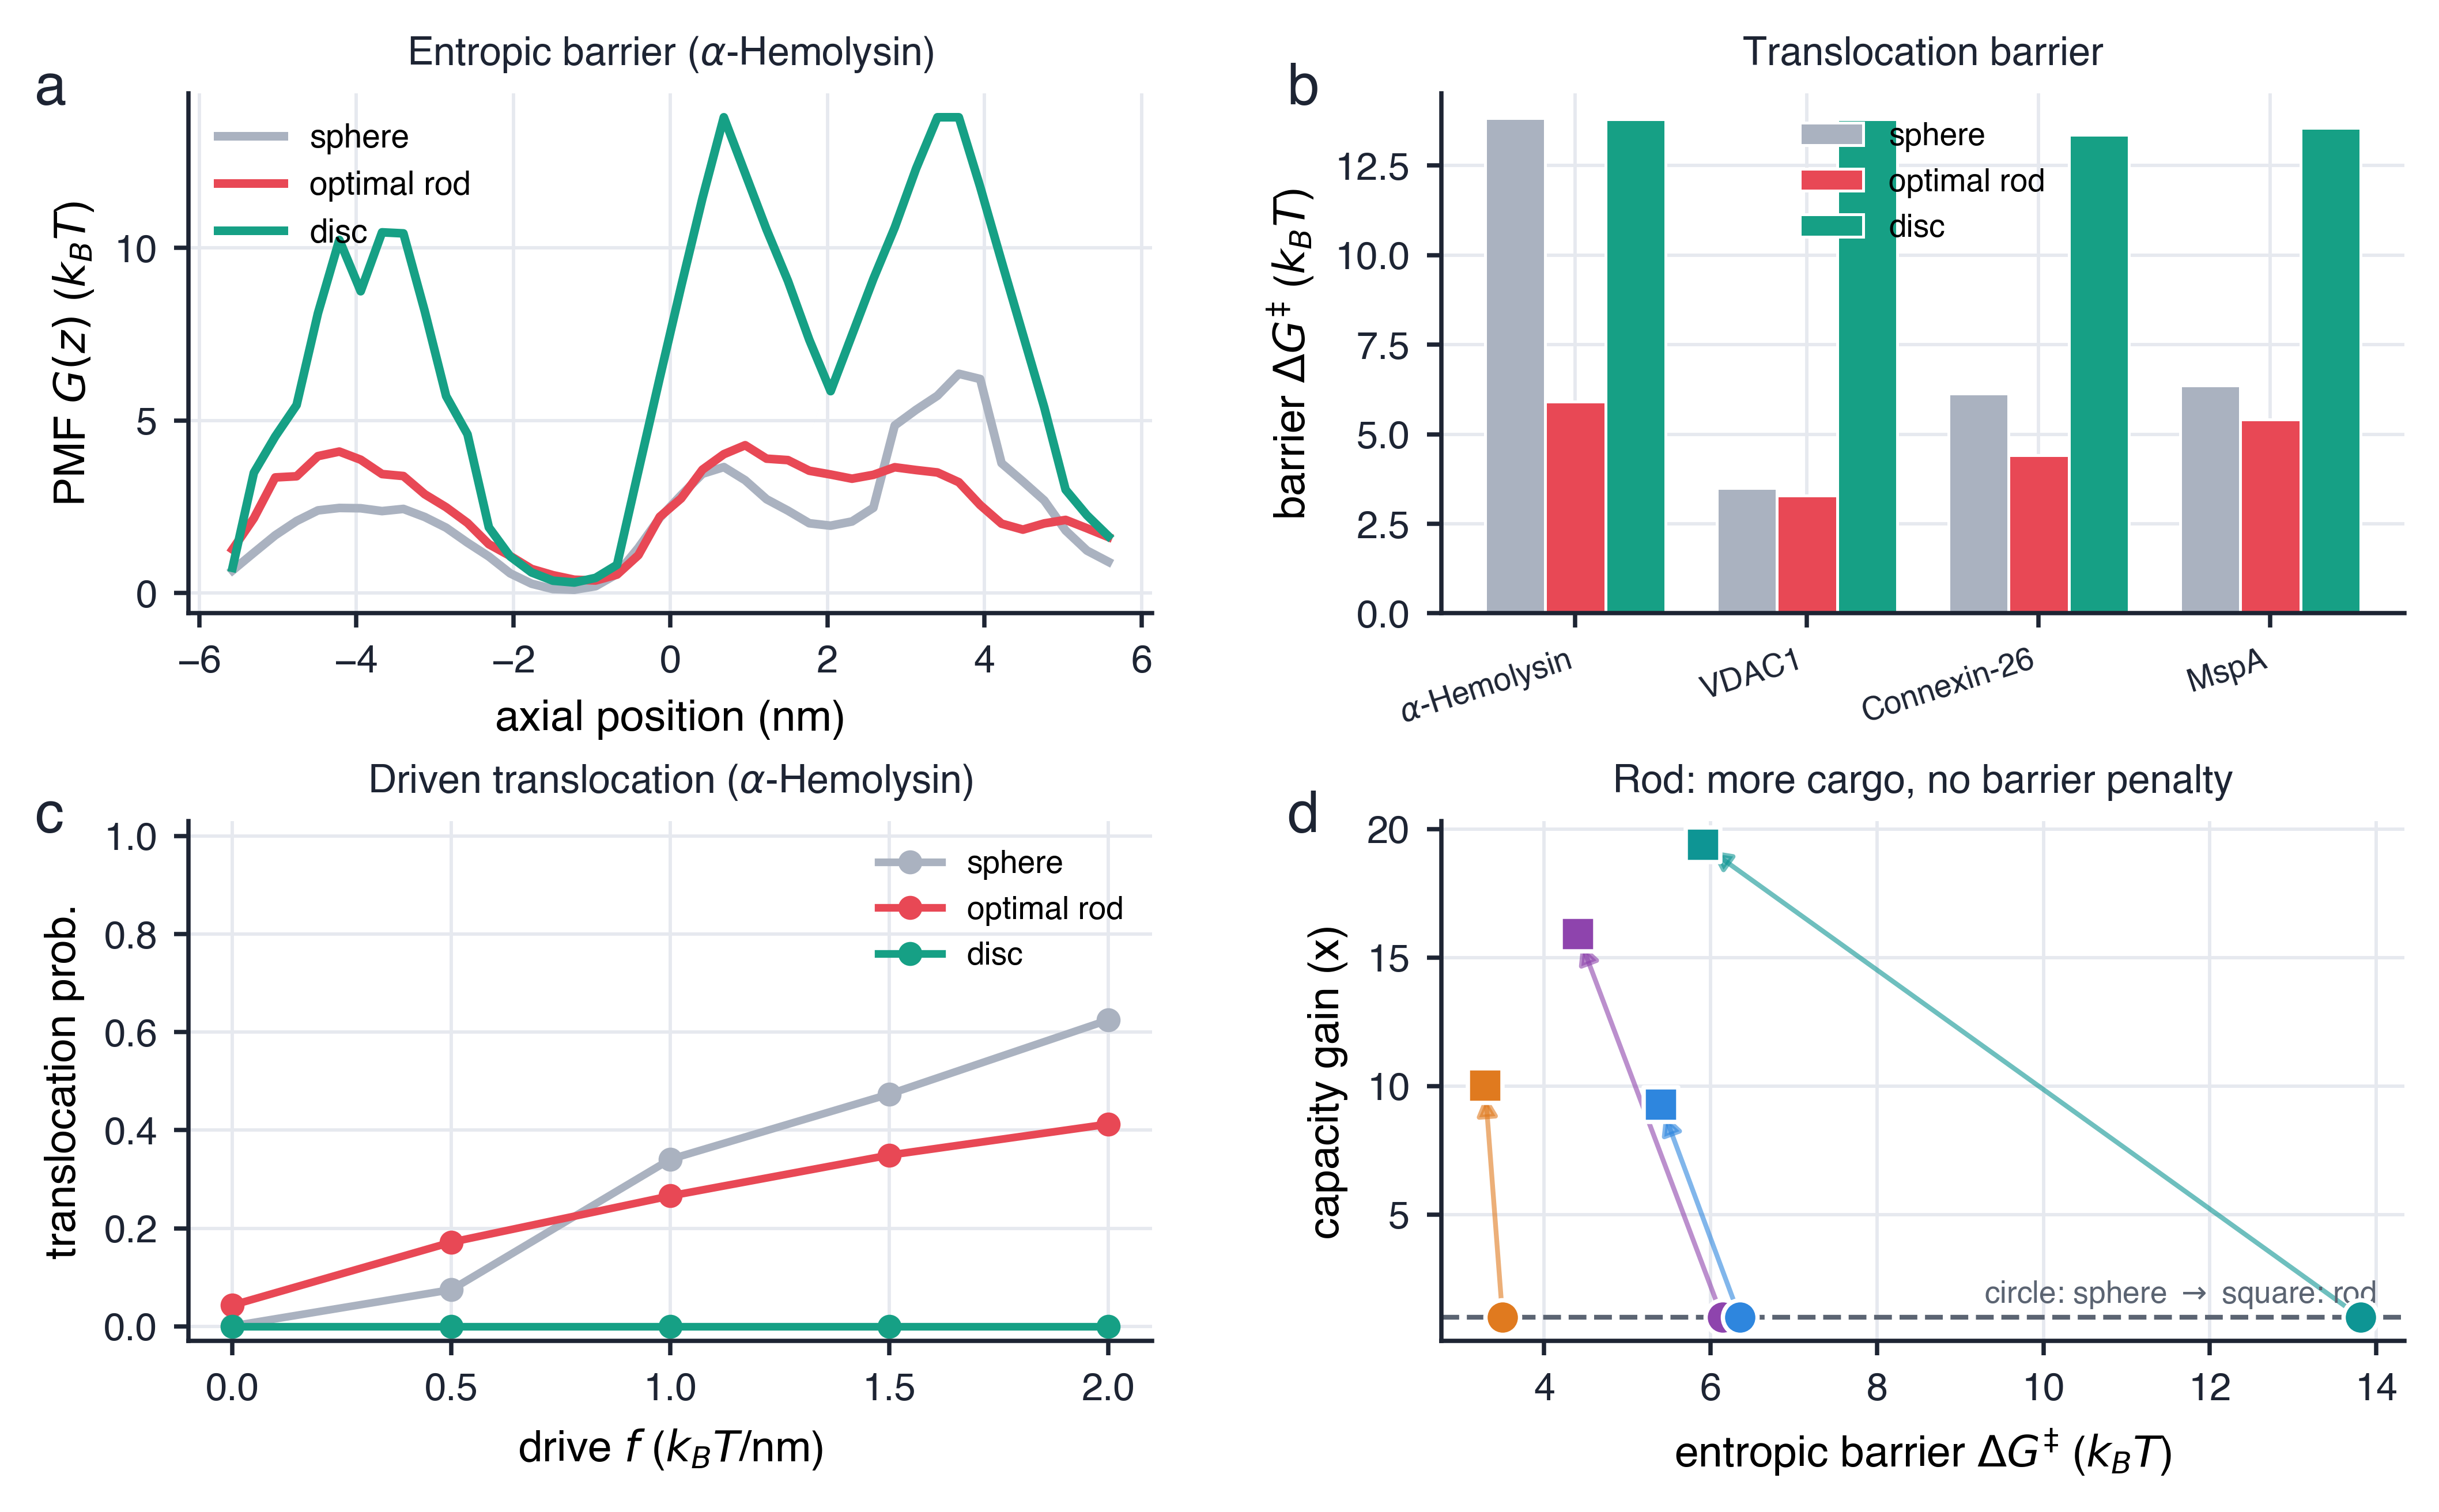
\includegraphics[width=\textwidth]{Figure7_brownian.png}
\caption{\textbf{Brownian-dynamics translocation.}
(a) Entropic PMF $G(z)$ for sphere, optimal rod and disc ($\alpha$-hemolysin).
(b) Peak translocation barrier per channel and shape; discs are blocked.
(c) Driven translocation probability versus applied force.
(d) Capacity gain versus translocation barrier: the sphere$\to$rod transition
(arrows) raises capacity by $\sim\!10$--$19\times$ with no barrier penalty.}
\label{fig:bd}
\end{figure*}

%====================================================================
\section{Mesoscale barriers and scale invariance}
\label{sec:meso}

Atomic-resolution nanopores are $\sim\!\SI{1}{nm}$ wide, whereas therapeutic
nanoparticles are typically $10$--$\SI{100}{nm}$. The dimensionless nature of the
capacity gain bridges this gap. Fixing the shape ratios and sweeping the absolute
pore radius over three decades leaves the gain exactly constant
(Fig.~\ref{fig:meso}a): the principle is scale-invariant, so the same
rod-beats-sphere (or disc-beats-sphere) logic applies from porins to micron-scale
tissue gaps.

Applying the framework with literature-informed descriptors of the major barriers
to delivery (Table~\ref{tab:meso}, Fig.~\ref{fig:meso}b) predicts capacity gains
of $1.4$--$4.3\times$ across the board: $4.1\times$ for claudin tight junctions
and $4.3\times$ for gap junctions (long, slit-like), $2.7\times$ for passive
nuclear-pore transport, $2.1$--$2.3\times$ for the tortuous mucus and collagen
meshes, and---because they are short, wide windows---$3.3\times$ for liver
fenestrae and $1.7\times$ for tumour vascular gaps, where the optimizer selects
oblate \emph{discs} ($a/R_{\rm bot}<1$) rather than rods. The shape that wins is
thus barrier-specific: rods for long channels, discs for short windows, with the
crossover dictated by the measurable length-to-radius ratio. This provides a
concrete, structure-aware design rule for the particle geometries that delivery
actually requires.

\begin{figure*}[t]
\centering
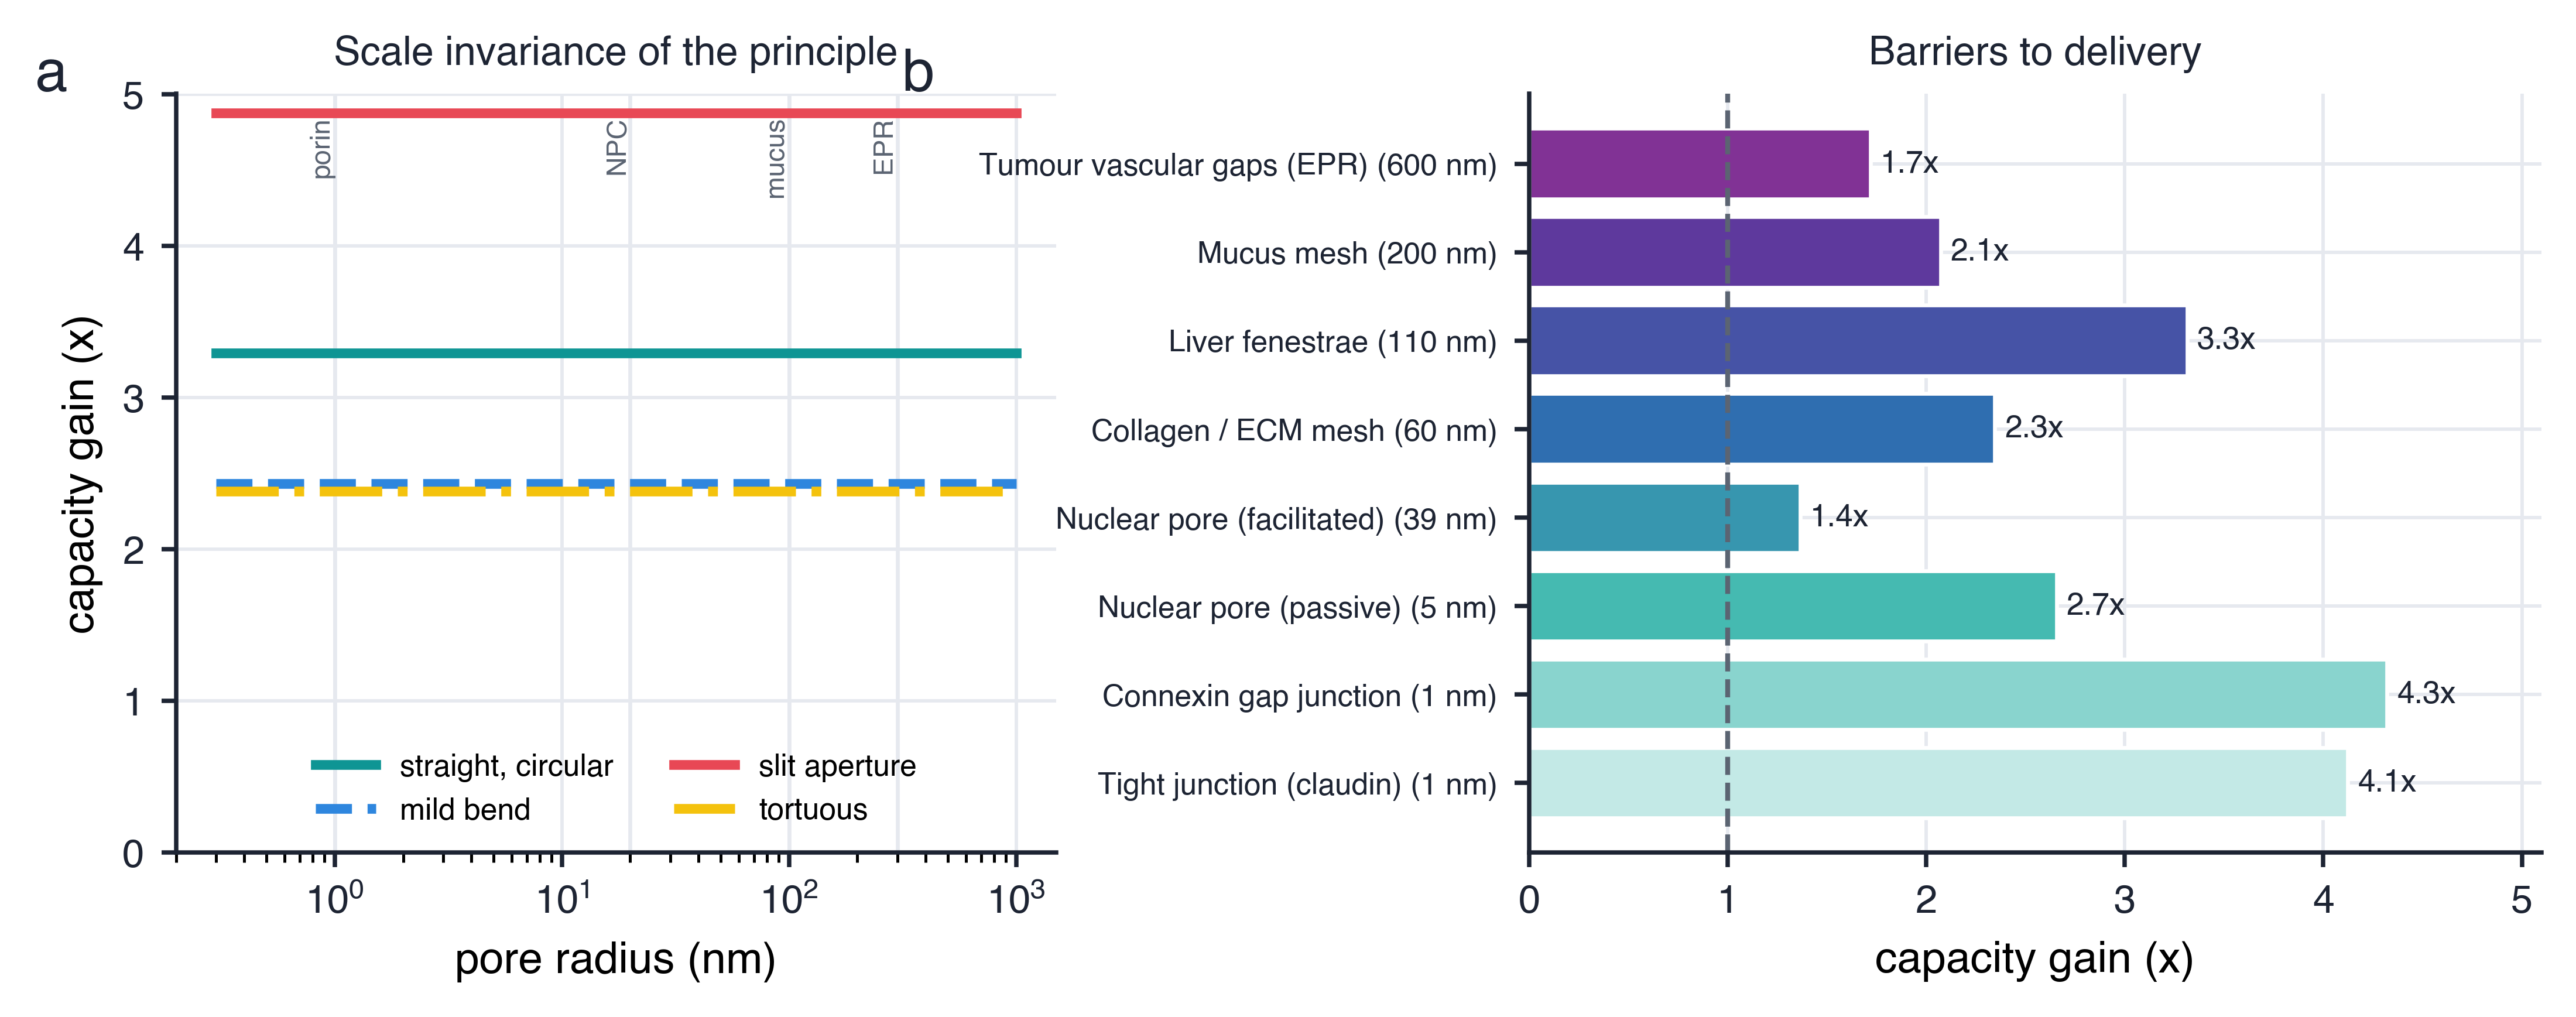
\includegraphics[width=\textwidth]{Figure8_mesoscale.png}
\caption{\textbf{Mesoscale extension and scale invariance.}
(a) For fixed shape ratios the capacity gain is independent of absolute pore
radius across three decades---the principle is scale-invariant.
(b) Predicted capacity gain for the major biological barriers to delivery; gains
exceed unity throughout, with rods favoured in long channels and discs in short,
wide windows.}
\label{fig:meso}
\end{figure*}

\begin{table}[t]
\caption{Mesoscale barriers to delivery: literature-informed descriptors and
predicted capacity gain $G$. $R$, constriction radius; $L$, traversal length;
$\tau$, tortuosity; $\epsilon_{\rm ap}$, aperture anisotropy. $a/R<1$ indicates a
disc-optimal regime.}
\label{tab:meso}
\begin{ruledtabular}
\begin{tabular}{lccccc}
Barrier & $R$ (nm) & $L$ (nm) & $\tau$ & $\epsilon_{\rm ap}$ & $G$ \\
\colrule
Tight junction (claudin)   & 0.35 & 4   & 1.05 & 2.5 & 4.1 \\
Gap junction (connexin)    & 0.6  & 15  & 1.10 & 1.5 & 4.3 \\
Nuclear pore (passive)     & 2.5  & 40  & 1.30 & 1.2 & 2.7 \\
Nuclear pore (facilitated) & 20   & 90  & 1.60 & 1.2 & 1.4 \\
Collagen / ECM mesh        & 30   & 300 & 1.80 & 1.6 & 2.3 \\
Mucus mesh                 & 100  & 800 & 2.00 & 1.5 & 2.1 \\
Liver fenestrae            & 55   & 60  & 1.05 & 1.3 & 3.3 \\
Tumour gaps (EPR)          & 300  & 400 & 1.20 & 1.4 & 1.7 \\
\end{tabular}
\end{ruledtabular}
\end{table}

%====================================================================
\section{Discussion}

Our central finding is that the rigid shape maximizing transportable cargo
through a molecular channel is not a sphere but a slender, round-cross-section
nanorod whose transverse size is set at the constriction and whose length is
bounded by a moving-sofa navigability limit. Across four canonical nanopores this
yields collision-validated capacity gains of an order of magnitude, governed by
the channel length-to-radius ratio and modulated by tortuosity. The optimum is
dynamically accessible---the rod translocates with no entropic-barrier penalty
relative to the maximal sphere---and the principle, being scale-invariant,
extends to the mesoscale barriers that limit drug delivery, where it predicts
rods for long channels and discs for short, wide windows.

These results rationalize and unify a body of experimental observations.
High-aspect-ratio carriers---filomicelles, nanorods and worm-like
micelles---circulate longer, penetrate barriers and reach the nucleus more
effectively than spheres \cite{geng2007,champion2006,kinnear2017,yang2010shape};
our framework supplies a geometric, capacity-based account of why elongation
helps, and quantifies how much. The disc/rod dichotomy we derive (discs for
short, wide or slit-like barriers; rods for long channels) offers a concrete,
structure-aware selection rule for the particle geometry best matched to a given
biological gate.

Several limitations bound the scope of the present, deliberately minimal, model.
(1) We treat particles and channels as rigid; deformability---central to the
passage of cells and soft liposomes through constrictions---would relax the
navigability bound and is a natural extension. (2) We resolve steric geometry
only; electrostatics (the Debye layer in physiological salt), hydration shells
and specific chemistry (e.g.\ the FG-nucleoporin mesh of the nuclear pore
\cite{tagliazucchi2013npc}) modulate real passage and would refine the effective
aperture. (3) The transportable volume is a geometric capacity, and the
Brownian-dynamics analysis an entropic, reduced-coordinate treatment; full
three-dimensional rigid-body dynamics and free-energy methods would sharpen the
kinetic predictions. (4) The mesoscale descriptors are order-of-magnitude,
literature-informed estimates rather than structure-derived. None of these
caveats affects the core geometric result, and each defines a concrete avenue for
refinement. We emphasize that the framework is fully reproducible and
structure-driven: every number derives from public coordinates through an open
pipeline, and the central predictions are checked by independent collision
detection.

The link to the moving-sofa problem is more than an analogy. The recent
resolution of Moser's problem \cite{baek2024} establishes that the area-maximal
navigating shape is anisotropic and corner-limited; our three-dimensional,
volume-maximizing, structure-resolved formulation transfers that lesson to
biophysics and turns it into a quantitative design tool. Beyond drug delivery,
the same geometry governs the rational design of biological and solid-state
nanopores for single-molecule sensing and sequencing \cite{manrao2012mspa,
kowalczyk2011nanopore}, where matching analyte shape to pore geometry is
paramount.

%====================================================================
\section{Methods}
\label{sec:methods}

\paragraph{Structures.} Coordinates were obtained from the Protein Data Bank
(7AHL, 3EMN, 2ZW3; MspA from the 1UUN biological octamer). Heavy atoms were
retained and assigned Bondi van der Waals radii \cite{bondi1964} via Biopython
\cite{cock2009biopython}.

\paragraph{Lumen geometry.} The pore axis was initialized from a cylinder fit
(minimizing the variance of atomic perpendicular distances) and refined to
maximize the enclosed lumen length. The inscribed-sphere radius was propagated
continuously along the axis from a central anchor using a bounded two-level grid
search, with an eight-sector enclosure test halting propagation at the pore
mouths, following the \textsc{hole} approach \cite{smart1996hole}. Tortuosity was
computed from the smoothed centreline; aperture anisotropy from directional
wall-clearance at the bottleneck.

\paragraph{Optimization.} Equation~\eqref{eq:opt} was solved by dense search over
$(\epsilon_1,\epsilon_2)$ and a transverse-scale/aspect parameterization, with
the transverse-fit constraint enforced by boundary sampling and the navigability
bound from Eq.~\eqref{eq:ladder}. The volume law \eqref{eq:volume} was validated
against $3\times10^6$-sample Monte-Carlo integration.

\paragraph{Atomistic validation.} The optimal particle's surface was discretized
and tested for overlap against all channel atoms (KD-tree nearest-atom queries)
as it was (i) grown radially at the bottleneck (transverse limit) and (ii)
elongated and swept along the lumen over a search of position and orientation
(navigable length). The largest collision-free configuration defines the
validated optimum.

\paragraph{Brownian dynamics.} The entropic PMF $G(z)=-k_BT\ln\Omega(z)$ was
estimated from the collision-free fraction $\Omega(z)$ of sampled rigid
configurations \cite{zwanzig1992}; overdamped Langevin trajectories were
integrated on $G(z)$ with absorbing boundaries to obtain translocation
probabilities and mean first-passage times. Figures were produced with
Matplotlib; molecular surfaces use marching cubes \cite{lorensen1987marching}.
SciPy \cite{virtanen2020scipy} provided optimization and spatial routines. All
code and derived data are available (see Data Availability).

%====================================================================
\section{Conclusions}

We have posed nanoparticle transport through a molecular channel as a
three-dimensional moving-sofa problem and solved it on real, atomistically
measured geometry. The optimal rigid carrier turns out to be a
navigability-limited nanorod. It holds an order of magnitude more cargo than the
largest sphere that fits, yet pays no penalty in translocation barrier. The same
argument is scale-invariant by construction, so it applies equally to
sub-nanometre porins and to micron-scale tissue gaps; the shape that wins simply
shifts from a rod in long channels to a disc in short, wide windows. What began
as a sixty-year-old geometry puzzle thus becomes a concrete design rule for
nanocarriers and for the engineering of biological and solid-state nanopores.

\begin{acknowledgments}
The author thanks the maintainers of the Protein Data Bank and the open-source
scientific Python ecosystem.
\end{acknowledgments}

\section*{Data availability}
All atomic coordinates are public (PDB 7AHL, 3EMN, 2ZW3, 1UUN). The analysis
pipeline, derived data and figure-generation code are available from the author
on reasonable request.

\appendix
\section{Verification of the superquadric volume law}
\label{app:volume}
Equation~\eqref{eq:volume} was checked against uniform Monte-Carlo integration
over the bounding box for representative shapes. For the sphere
($\epsilon_1=\epsilon_2=1$, $r_x=r_y=c=1$) the formula gives $4.189$ versus
$4.189$ (Monte-Carlo) and the exact $\tfrac{4}{3}\pi=4.18879$; for a prolate
ellipsoid, a unit cylinder, a flat disc and a short cylinder the formula and
Monte-Carlo agree to better than $0.1\%$. An alternative single-exponent
parameterization with the commonly mis-stated prefactor over-counts volume by a
factor that grows with the exponent (e.g.\ $2.0\times$ at $n=2$, $6.8\times$ at
$n=3$), which would spuriously favour boxy shapes; we therefore use the
verified two-exponent law throughout.

\bibliographystyle{apsrev4-2}
\bibliography{references}

\end{document}
